\documentclass[a4paper,11pt]{article}
\usepackage[utf8]{inputenc}
\usepackage[T1]{fontenc}
\usepackage{lmodern,amsmath,amssymb,graphicx,booktabs,longtable,array}
\usepackage[margin=24mm]{geometry}
\usepackage{microtype}
\usepackage{xr-hyper}
\usepackage[colorlinks=true,linkcolor=blue,citecolor=blue,urlcolor=blue,pdfauthor={Finn Hinrichsen},pdftitle={Radiative cancellations and localized linear modes in three-dimensional sextic Q-balls}]{hyperref}
\externaldocument[][nocite]{supplement}
\setlength{\emergencystretch}{2em}
\newcommand{\dd}{\mathrm{d}}
\newcommand{\ii}{\mathrm{i}}
\newtheorem{conjecture}{Conjecture}
\title{Radiative cancellations and localized linear modes\\in three-dimensional sextic Q-balls}
\author{Finn Hinrichsen}
\date{30 October 2026 --- Preprint 0.53}
\begin{document}
\maketitle
\begin{center}
{\small\emph{To my parents, who told me that small steps of learning add up.}}
\end{center}
\begin{abstract}
We study localized linear excitations of a classical complex scalar Q-ball in three
spatial dimensions with potential $\mathcal U(S)=S-S^2+S^3/2$.
In a regime with one propagating and one evanescent exterior channel,
we assemble computer-assisted existence arguments for two radial modes
and one dipole mode on the infinite radial domain. Analytic exterior
estimates and ball-arithmetic interior enclosures distinguish these
results from finite-box linewidth minima. A numerical radial sequence,
with candidates reported through index eighteen, motivates a thin-wall
phase-matching description. An independently computed planar transmission
zero yields an unfitted spacing candidate; identifying this value with
a radial limiting spacing remains open. A second-harmonic analysis
separates one dipole monopole outgoing coefficient from zero under
explicitly audited exact-mode and enclosure hypotheses. It obstructs a
specified uniformly localized smooth continuation for every linked dipole
polarization with $\boldsymbol p^T\boldsymbol p\ne0$; circular polarization
requires a separate quadrupole certificate. Linear existence, numerical
spacing and nonlinear continuation are treated as distinct statements.
\end{abstract}

\section{A non-technical overview}\label{sec:overview}
This section explains the setting and the main statements without
technical prerequisites. Figure~\ref{fig:overview} summarizes it in one
picture. The precise statements, their evidence and their limits are
those of the later sections; nothing here adds a result.

\paragraph{What is a Q-ball?}
A Q-ball is a lump of a field that holds itself together. The field in
this paper is a complex scalar field, a quantity with a size and an
internal phase at every point of space. In a Q-ball the size forms a
round, localized profile, while the internal phase turns steadily in
time, like the hand of a clock with angular frequency~$\omega$. The
density of the field, and therefore the shape of the lump, does not
change in time (Fig.~\ref{fig:overview}a). The rotation carries a
conserved charge~$Q$, which plays the role of a particle number.
Coleman showed that, in suitable theories with such a conserved charge,
lumps of sufficiently large charge have less energy than the same charge
carried by free particles; such lumps cannot simply fall apart and are
stable~\cite{Coleman1985}. This general argument concerns large charge;
the stability of the particular backgrounds of this paper is not
established here. Friedberg, Lee and Sirlin had earlier constructed related
nontopological solitons, which also rely on a conserved additive quantum
number, in a model with an additional neutral
field~\cite{FriedbergLeeSirlin1976}. Q-balls with a large charge have a
nearly uniform interior and a transition zone of fixed thickness at the
surface~\cite{Coleman1985}. In the present model this thin-wall regime
is reached as $\omega^2$ approaches $1/2$; the wall keeps its thickness
while the radius grows, so the wall becomes thin relative to the ball.

\paragraph{What holds it together?}
The shape follows from a balance of competing tendencies. Gradients cost
energy, so the field profile is smoothed and any edge is softened. Far
outside, the field decays to zero because of its mass and because
$\omega^2<1$. The potential $\mathcal U(S)=S-S^2+S^3/2$ of the field
density $S=|\phi|^2$ contains a negative term $-S^2$, which lowers the
energy relative to free, non-interacting field, and a positive term
$S^3/2$, which penalizes high density. At fixed conserved charge this
combination permits binding; in the thin-wall regime the preferred
interior density tends to $S=1$. Coleman gave an intuitive picture of
this balance~\cite{Coleman1985}: the equation for the radial profile is
the equation of motion of a particle whose position is the field value
and whose time is the radius. The particle moves in a landscape with two
hills and is slowed by a damping term that becomes weaker at large
radius (Fig.~\ref{fig:overview}b). A Q-ball corresponds to a particle
that starts at rest on the inner side of the outer hill and comes to
rest exactly on the hill at zero field. For the present potential this
is possible only for $1/2<\omega^2<1$. Close to $\omega^2=1/2$ the two
hills have almost equal height; the particle then starts very close to
the top and lingers there, which gives a large uniform core with a
comparatively thin wall.

\paragraph{Vibrations, two channels and radiation.}
A Q-ball can vibrate. A small vibration with frequency $\rho$ of the
rotating lump appears in the field at two partner frequencies,
$\omega+\rho$ and $\omega-\rho$; these coupled sidebands are the standard
description of Q-ball perturbations~\cite{Kovtun2018}. Far from the
ball, a component can travel outwards as a wave only if the magnitude of
its frequency exceeds one, the mass of the field in our units; below
that threshold its tail decays exponentially. A negative frequency, as
for $\omega-\rho$ here, only means that the phase turns the other way.
In the regime studied here one partner lies above the threshold and the
other below it (Fig.~\ref{fig:overview}c). The upper partner is an open
channel: it can carry energy away to infinity as radiation. The lower
partner is a closed channel: it is trapped near the ball. Excited
Q-balls have vibrational modes~\cite{Kovtun2018}, and in a
one-dimensional version of the same type of model a squashed Q-ball
relaxes by radiating through such channels~\cite{Ciurla2024}. A typical
vibration in our regime should therefore leak energy and fade. Its
leakage rate is measured by the width of the resonance: the larger the
width, the faster the vibration fades.

\paragraph{When the radiation vanishes.}
How much energy leaks depends on the amplitude of the outgoing wave in
the open channel. Contributions to this wave from different parts of
the ball can cancel each other by interference. When they cancel
completely, the width is zero and the vibration stays exactly localized
although a radiation channel is open. Such a state is a bound state in
the continuum (BIC): a localized wave that coexists with extended waves
of the same frequency but does not radiate~\cite{Hsu2016}. The idea was
proposed in quantum mechanics as early as 1929 by von Neumann and
Wigner, and BICs have since been studied in many wave systems,
particularly in photonics; one known route is the cancellation of
radiating components, for example when two interacting resonances
interfere so that the width of one of them
vanishes~\cite{Hsu2016,FriedrichWintgen1985}.
Figure~\ref{fig:overview}d shows the computed mode C0: its open-channel
component decays like the trapped one instead of leaving an outgoing
tail.

\paragraph{Why this is not automatic.}
Three reasons make such cancellations nontrivial. First, once the
background and the overall size of the vibration are fixed, the outgoing
wave must vanish in both of its oscillation phases. These are two real
matching conditions for the two frequencies $\omega$ and $\rho$.
Generically this suggests that cancellations, if they occur, sit at
isolated parameter points that have to be found. The proofs below
establish existence inside small parameter boxes; they do not establish
that the parameter pair is unique. Second, for a single wave scattered
by an object of finite extent, such trapped states are generally
excluded~\cite{Hsu2016}. The Q-ball problem is of a different kind: the
vibration has two coupled components, one of which cannot propagate.
For the linearization about the ground state of the focusing cubic
nonlinear Schr\"odinger equation in three dimensions, embedded
eigenvalues are proved to be absent~\cite{LiYang2026}; the present
relativistic model is different, and nothing here contradicts that
theorem. Third, a computer calculation in a finite box can show a very
small width that is not exactly zero. Only a proof that controls the
infinite exterior separates an exact zero from a near miss. This is the
reason for the computer-assisted proofs in
Section~\ref{sec:certified-existence}. They use interval arithmetic,
which carries guaranteed bounds through every rounded arithmetic
operation, together with analytic estimates that bound the remaining
approximation errors and the infinite exterior.

\paragraph{Proved cancellations and numerical candidates.}
Figure~\ref{fig:overview}e and Fig.~\ref{fig:ladder} show where
cancellations of the spherically symmetric vibrations have been proved
or numerically located. Eighteen locations are reported, labelled
$n=1,\ldots,18$; they move from $\omega^2\approx0.798$ towards the
thin-wall threshold $\omega^2=1/2$. Only the first two, C0 and C1, are
exact zeros established by computer-assisted proofs with analytic control
of the infinite exterior. A third proof, C2, concerns a dipole vibration,
in which two opposite halves of the ball oscillate against each other;
it belongs to a separate angular channel. The other sixteen locations
are numerical candidates, for which an exact zero is not established,
with the graded evidence of Table~\ref{tab:ladder}. For $n=3$--$15$ a
numerical winding test was resolved: the two matching errors were seen
to circle zero once around the candidate (for $n=5$ and $11$--$14$ in a
calculation added in this revision), and $n=16$--$18$ failed the final
acceptance rule. Figure~\ref{fig:overview}e still marks $n=5$ and
$11$--$14$ with the weaker evidence classes of preprint 0.52; their
location changes are below its plotting resolution. The inverse detuning $1/(\omega^2-1/2)$ measures how
close a ball is to the thin-wall threshold. Plotted against it, the
locations are nearly equally spaced; between indices 12 and 15 the steps
are about $2.30$ to $2.31$. In the thin-wall picture this has a simple
reading. The radius of the ball grows in proportion to the inverse
detuning, Eq.~\eqref{eq:thinwall}. The interior acts like a resonator
between the centre and the reflecting wall, and a further cancellation
appears whenever one more half wavelength fits into the interior
(Section~\ref{sec:thinwall}). This finite-radius phase description is
partly calibrated to the numerical results. If the interior wavelength
and the phase at the wall approach limits, it suggests approximately
equal steps; it is not a parameter-free prediction of all locations.
A separate calculation for a flat wall, not fitted to the locations,
gives a candidate value $2.3100$ for the step.

Several things are not shown. There is no proof of an infinite
ladder, and the identification of the flat-wall value with the actual
limiting step remains open; a frozen formula for the absolute locations
failed its test. The stability of the Q-ball backgrounds themselves is
not established. A numerical check of how the charge changes with the
frequency bears, under the assumptions of a standard criterion, only on
one simple kind of instability, a purely growing radial deformation, and
finds no sign of it (Section~\ref{sec:discussion}). Finally, the cancellation is a statement about small,
linear vibrations. At finite amplitude, nonlinear terms can drive second
harmonics, with laboratory frequencies $\omega\pm2\rho$; for the
certified modes these lie in the propagating range, but this alone does
not establish outgoing radiation. For the dipole mode C2, under stated
hypotheses, one outgoing second-harmonic coefficient is guaranteed to be
nonzero. This obstructs a specified smooth localized continuation to
finite amplitude, while circular polarization needs a separate
certificate (Section~\ref{nl:section}). For C1 the corresponding
calculation is open. The linear trapping found here therefore does not
establish a nonlinear trapping, and no lifetime or instability is
inferred.

\paragraph{Potential significance.}
The following points are possibilities for further work, not claims of
this paper. Numerical simulations indicate that Q-balls can form in
the early universe through the fragmentation of an Affleck--Dine scalar
condensate~\cite{KasuyaKawasaki2000}, and supersymmetric Q-balls have
been proposed as a contribution to dark
matter~\cite{KusenkoShaposhnikov1998}. Whether comparable linear
cancellations occur in such models, and whether they matter for how
long internal vibrations last, are open questions; the present model,
its parameters and the nonlinear limitation noted above support no
statement about lifetimes or observations. In photonics, BICs underlie
sharp resonances with high quality factors; in real structures of
finite size they appear as quasi-BICs, weakly leaking approximations to
an ideal BIC~\cite{Koshelev2018}, with applications ranging from lasers
and sensors to filters~\cite{Hsu2016}. The Q-ball zeros share the
interference and resonator logic of such systems; this is an analogy of
mechanism, and no experimental realization is proposed. Finally, the
combination of interval arithmetic with analytic control of the
infinite exterior used here is a general method: it can separate exact
embedded eigenvalues from small numerical widths in other soliton
problems, in the spirit of related computer-assisted spectral
work~\cite{LuhrmannEtAl2026,MarzuolaSimpson2011}. None of this amounts
to a stability result, a particle model or an experimental proposal.

\begin{figure}[p]\centering
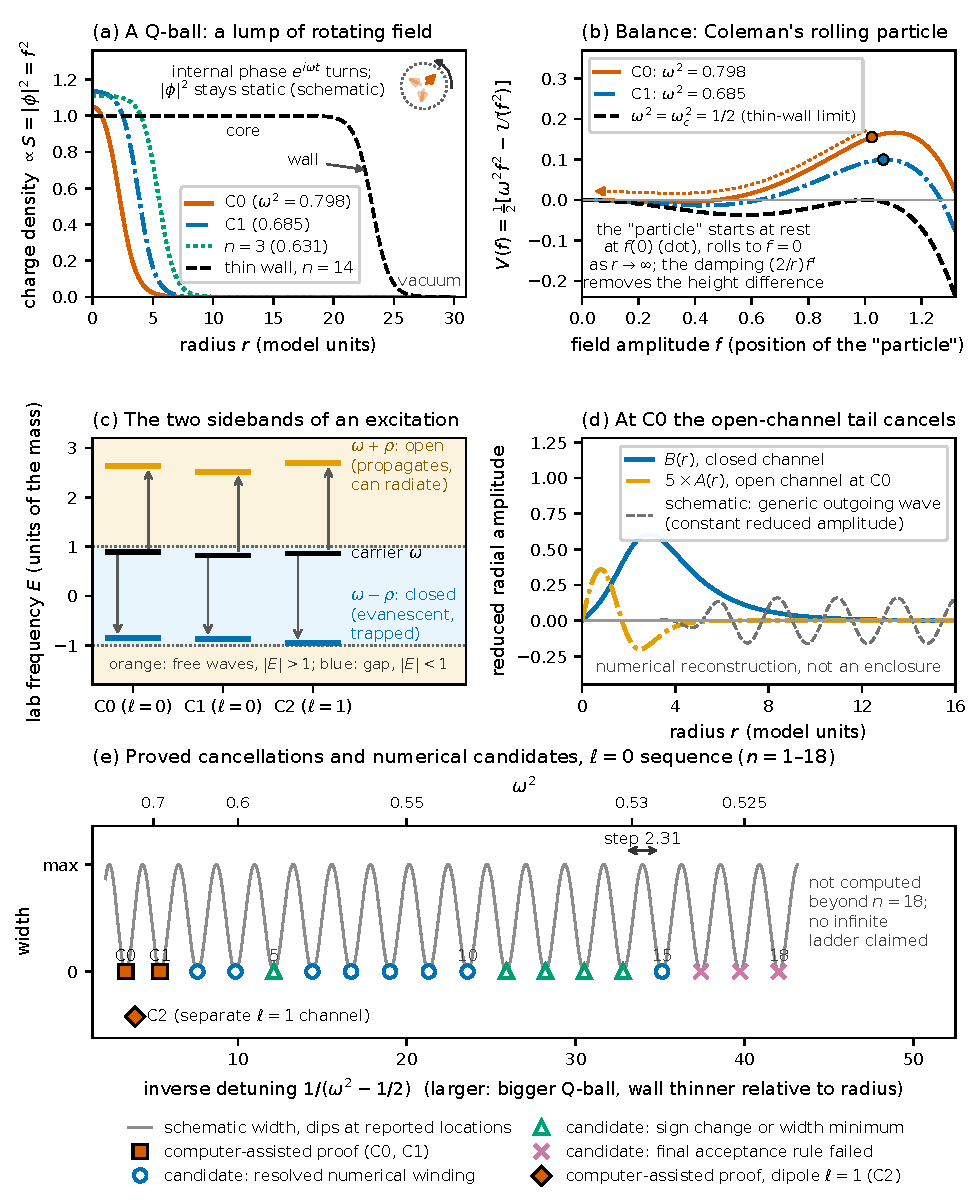
\includegraphics[width=.95\linewidth]{qball-overview.pdf}
\caption{Overview of the objects studied in this paper.
(a)~Density profiles $S=f^2$ of stored backgrounds (C0, C1, $n=3$) and
the leading thin-wall formula, Eq.~\eqref{eq:thinwall}, at the
$\omega^2$ of index $14$; the inset is schematic.
(b)~Coleman's mechanical picture of Eq.~\eqref{eq:profile}~\cite{Coleman1985}
with $V(f)=\frac12[\omega^2f^2-\mathcal U(f^2)]$; dots mark the stored
central values $f(0)$.
(c)~Sideband frequencies $\omega\pm\rho$ of the three certified modes
(Table~\ref{tab:proof-cases}) relative to the threshold $|E|=1$ of
Eq.~\eqref{eq:channels}.
(d)~Stored numerical reconstruction of the C0 channel functions, not a
pointwise enclosure. $A=ra$ and $B=rb$ remove the $1/r$ spreading, so
the schematic outgoing wave has constant reduced amplitude while its
physical field falls as $1/r$.
(e)~Locations of Table~\ref{tab:ladder} and of C2 on the inverse-detuning
axis, marked by evidence class (preprint 0.52). The grey width curve is schematic: its
dips are placed at the reported locations, and a zero depth is
established only for C0, C1 and C2. The step label is the difference
between indices 14 and 15; nothing beyond $n=18$ is computed or implied.
Sources and checksums: Section~\ref{app:provenance}.}
\label{fig:overview}
\end{figure}


\section{Question and scope}\label{sec:scope}
A small resonance width, an exactly localized linear mode and a localized
finite-amplitude oscillation require different evidence. We examine this
separation for a complex scalar Q-ball, reporting three existence
enclosures, a broader numerical sequence and a wall-scattering
interpretation of its spacing. The sequence label $n$ is a continuation
index, not a certified node count or a completeness statement.
A bound state in the continuum (BIC) denotes a localized linear mode in
an available propagating-channel regime~\cite{Hsu2016}. Uncertified
locations will be called candidates. All quantities are dimensionless.
\subsection{Relation to Q-ball excitations and continuum trapping}
\label{sec:related-work}

Q-balls are localized scalar configurations carrying a conserved global
charge~\cite{Coleman1985}. Battye and Sutcliffe study collisions, charge
transfer and fission in one, two and three spatial dimensions in the same
sextic model, after unit conversion~\cite{BattyeSutcliffe2000}.
Kovtun, Nugaev, and Shkerin formulate the coupled sideband problem
$\omega\pm\rho$ and analyze three-dimensional vibrational
modes~\cite{Kovtun2018}. Azatov, Ho, and Khalil treat scattering in the
sextic family, as well as the complex-plus-real-field
Friedberg--Lee--Sirlin model~\cite{Azatov2024,FriedbergLeeSirlin1976}.
The coupled radial operator is established prior work; the contribution
here concerns particular localized solutions of it, with regular origin
conditions and controlled infinite tails.

Chen, Andersson, and Li analyze three-dimensional Q-ball perturbations
for the rescaled potential $V(s)=s^2-s^3+\kappa s^4$, where $s$ denotes
the field modulus~\cite{ChenAnderssonLi2025}. Their coupled-sideband
classification provides context, but concerns a different potential.
Our claim is the certification of three particular localized linear
modes of the sextic model, including cancellation of both oscillatory
open-channel components. Among the works reviewed here, we did not
identify a predecessor for these specific modes. This limited
statement establishes neither global priority nor a contradiction with
the spectrum studied by Chen and collaborators.

Zhang, Zhou, and Zhu obtain analytic scattering solutions from stepwise
Q-ball profiles~\cite{ZhangZhouZhu2025}. Their interior dispersion and
thin-wall phase structure are directly relevant to Eq.~\eqref{eq:interior},
although their propagating scattering regime has two exterior open
channels. Ciurla et al. distinguish bound, half-propagating and quasinormal
modes in $1+1$ dimensions~\cite{Ciurla2024}. Their half-propagating interval
$1-\omega<\rho<1+\omega$ has the same channel thresholds as ours, but their
long-lived example retains a small radiative tail. Evslin et al. analyze
paired Floquet modes of small-amplitude, one-dimensional
Q-balls~\cite{Evslin2026}; coupling of a discrete component to its
propagating partner produces Feshbach-type quasinormal modes. These
one-dimensional calculations do not transfer the spherical origin
condition or radial measure to three dimensions.

Numerically assisted spectral exclusion arguments for NLS solitary waves
include those of Marzuola and Simpson and Asad and
Simpson~\cite{MarzuolaSimpson2011,AsadSimpson2011}.
Cuccagna and Maeda impose absence of embedded eigenvalues as hypothesis H4
and describe the broader ground-state expectation as unproved in their
2020 survey~\cite[Remark 3.2]{CuccagnaMaeda2020}.
Li and Yang subsequently prove absence in the essential spectrum for the
full linearized operator about the ground state of the three-dimensional
focusing cubic NLS~\cite[Theorem 1.1]{LiYang2026}. This is a different
equation and operator from our relativistic Q-ball frequency pencil.
A nodeless Q-ball profile alone does not establish the relevant
variational ground-state class. The present model-specific existence
claim therefore does not contradict that NLS theorem or refute the
survey's expectation in its stated setting.

A bound state in the continuum (BIC) is a spatially localized linear state
at a frequency also admitting extended radiation modes~\cite{Hsu2016}.
Interference-induced trapping is an established mechanism:
Friedrich and Wintgen relate interacting resonances to vanishing decay
width~\cite{FriedrichWintgen1985}, and Yu and Lu give an existence theorem
for a three-channel Schr\"odinger problem with one open
channel~\cite{YuLu2025}. Its small-coupling assumptions and finite-range
potential differ from the present two-channel pencil with an infinite
profile tail. Related resonant reflection occurs for discrete breathers,
optical solitons and condensate domain
walls~\cite{Flach2003,Flach2005,Watabe2012}.

Winding numbers for BICs are also established: Zhen et al. use the winding
of a real far-field polarization vector in the two-dimensional Bloch
wave-vector plane of a photonic slab~\cite{Zhen2014}. Their symmetry
assumptions support a charge-conservation and robustness statement.
Our winding of a matching map over Q-ball parameters is a numerical
zero-finding diagnostic; it does not inherit that photonic robustness
theorem.

The planar transmission zero and interior phase matching admit a
\emph{Fabry--P\'erot interpretation}. Hsu et al. describe BICs formed by
perfect resonant reflection together with a round-trip phase condition,
including a resonator paired with a reflecting boundary~\cite{Hsu2016}.
In the thin-wall picture used here, the reflecting wall and the regular
centre supply the analogous radial cavity. This is an interpretation of
the wall and phase calculations, rather than an additional existence
result for the curved Q-ball. In particular, the planar zero alone does
not certify a spherical mode. Sequences of radiation cancellations and
WKB matching are also known for nonlinear embedded
solitons~\cite{Malomed2005}; their model and scaling parameter differ from
those of the present sequence of linear modes on changing backgrounds.

Nonlinear radiation obstructions have a separate history. Segur and
Kruskal find beyond-all-orders radiation excluding small-amplitude true
breathers in the one-dimensional $\phi^4$
model~\cite{SegurKruskal1987}. Sigal studies instability of periodic and
quasiperiodic wave solutions under generic nonlinear
perturbations~\cite{Sigal1993}; Soffer and Weinstein prove radiation
damping under a Fermi-golden-rule hypothesis~\cite{SofferWeinstein1999}.
Manton and Merabet derive second-harmonic radiation with amplitude of
order $A^2$ and power of order $A^4$ from a kink's internal mode in
$1+1$-dimensional $\phi^4$ theory~\cite[Appendix A]{MantonMerabet1997}.
The harmonic mechanism and power counting are known; their coefficients
and perturbative decay law are not transferred to our three-dimensional
Q-ball.
The present contribution in this direction is the explicit error budget
separating a particular second-harmonic coefficient from zero. Its
continuation obstruction has the stated hypotheses and is not a
dynamical decay theorem. Oscillon decay minima~\cite{ZhangOscillons2020}
and the second-harmonic radiation zeros of a critical-bubble internal
mode~\cite{InagakiMurakami2026} further illustrate why suppression at one
harmonic does not establish an exactly localized nonlinear oscillation.

L\"uhrmann et al. combine analytic estimates and interval arithmetic to
certify vortex profiles, spectral data and nonzero Fermi-golden-rule
coefficients in the self-dual abelian Yang--Mills--Higgs model in two
spatial dimensions~\cite[Theorem 1.1, Remark 1.2 and Section 2]{LuhrmannEtAl2026}.
Their internal mode is a gap eigenvalue. This is a methodological
precedent for rigorous spectral and radiation-coupling computations.
Here the distinct target is a particular outgoing second-harmonic
coefficient associated with a localized linear Q-ball mode in three
dimensions. Its conditional continuation obstruction remains separate
from a nonlinear decay, lifetime or background-stability theorem.

Background stability is likewise distinct from mode localization.
Classical stability results for charged scalar solitons and the
Vakhitov--Kolokolov slope criterion provide the appropriate
context~\cite{FriedbergLeeSirlin1976,VakhitovKolokolov1973}.
Applying such a criterion requires its model-dependent hypotheses and
charge convention; the certificates here do not determine $dQ/d\omega$
at the three backgrounds. A numerical evaluation and its limited scope
are given in Section~\ref{sec:discussion}. The literature comparisons delimit the claimed
contribution without establishing exhaustive priority or an infinite
ladder.


\section{Field model and two-channel linearization}\label{sec:model}
With metric signature $(+,-,-,-)$, define
\begin{equation}\label{eq:action}
\mathcal L=\partial_\mu\phi^*\partial^\mu\phi-\mathcal U(|\phi|^2),
\qquad \mathcal U(S)=S-S^2+\beta S^3,\qquad \beta=\tfrac12.
\end{equation}
The free scalar mass is one. A spherical stationary background is
$\phi_0=e^{\ii\omega t}f(r)$ with real $f$, satisfying
\begin{equation}\label{eq:profile}
f''+\frac2r f'=(1-\omega^2)f-2f^3+3\beta f^5,
\quad f'(0)=0,\quad f(r)\longrightarrow0.
\end{equation}
For definiteness the charge sign is chosen so that
$Q=2\omega\int f^2\dd^3x>0$ when $\omega>0$.
The thin-wall frequency threshold is
$\omega_c^2=\min_{S>0}\mathcal U(S)/S=1-1/(4\beta)=1/2$.

Use a real orthonormal spherical-harmonic basis and write
\begin{equation}\label{eq:ansatz}
\delta\phi=e^{\ii\omega t}
 [a(r)e^{\ii\rho t}+b(r)e^{-\ii\rho t}]Y_{lm}(\hat x),
\qquad A=ra,\quad B=rb,
\end{equation}
for real-frequency, real-radial-function modes. In a complex harmonic basis
the second sideband instead carries $Y_{lm}^*$.
Let $S=f^2$, $D=1-4S+9\beta S^2$, and $C=-2S+6\beta S^2$.
The radial equations are
\begin{align}
 A''&=\left[D+\frac{l(l+1)}{r^2}-(\omega+\rho)^2\right]A+CB,
 \label{eq:radialA}\\
 B''&=CA+\left[D+\frac{l(l+1)}{r^2}-(\omega-\rho)^2\right]B.
 \label{eq:radialB}
\end{align}
Regular solutions satisfy $A,B=O(r^{l+1})$ at the origin.
In the range $1-\omega<\rho<1+\omega$, define
\begin{equation}\label{eq:channels}
k^2=(\omega+\rho)^2-1>0,\qquad
\kappa_c^2=1-(\omega-\rho)^2>0,\qquad
\kappa_0^2=1-\omega^2>0.
\end{equation}
The $A$ channel is open and the $B$ channel closed. A localized mode
requires cancellation of both oscillatory exterior components of $A$
and exclusion of the growing component of $B$.
The asymptotic continuous-frequency branches start at $|\rho|=1-\omega$,
with the second channel opening at $|\rho|=1+\omega$; these are the
standard Q-ball sideband thresholds~\cite{Kovtun2018,Ciurla2024}.
Here ``embedded'' specifies an exactly localized solution in this
continuous-frequency range. The certificates establish a partial-wave
statement, rather than a separate theorem about the full evolution
generator's essential spectrum or algebraic multiplicity.

The spatial dimension is three; the two sidebands are field components,
not additional spatial dimensions. Spherical reduction retains the
three-dimensional measure and centrifugal term. It is neither a
one-dimensional field theory nor a test of all three-dimensional
perturbations. In one spatial dimension there is no spherical centrifugal
term; in two dimensions both the radial measure and angular decomposition
change. The planar wall below is a local thin-wall approximation to the
three-dimensional profile. The separate two-dimensional numerical study
is retained in the Supplement; profiles and charge normalizations are
not transferred between dimensions. Higher spatial dimensions are outside
the present evidence.

\begin{figure}[htbp]\centering
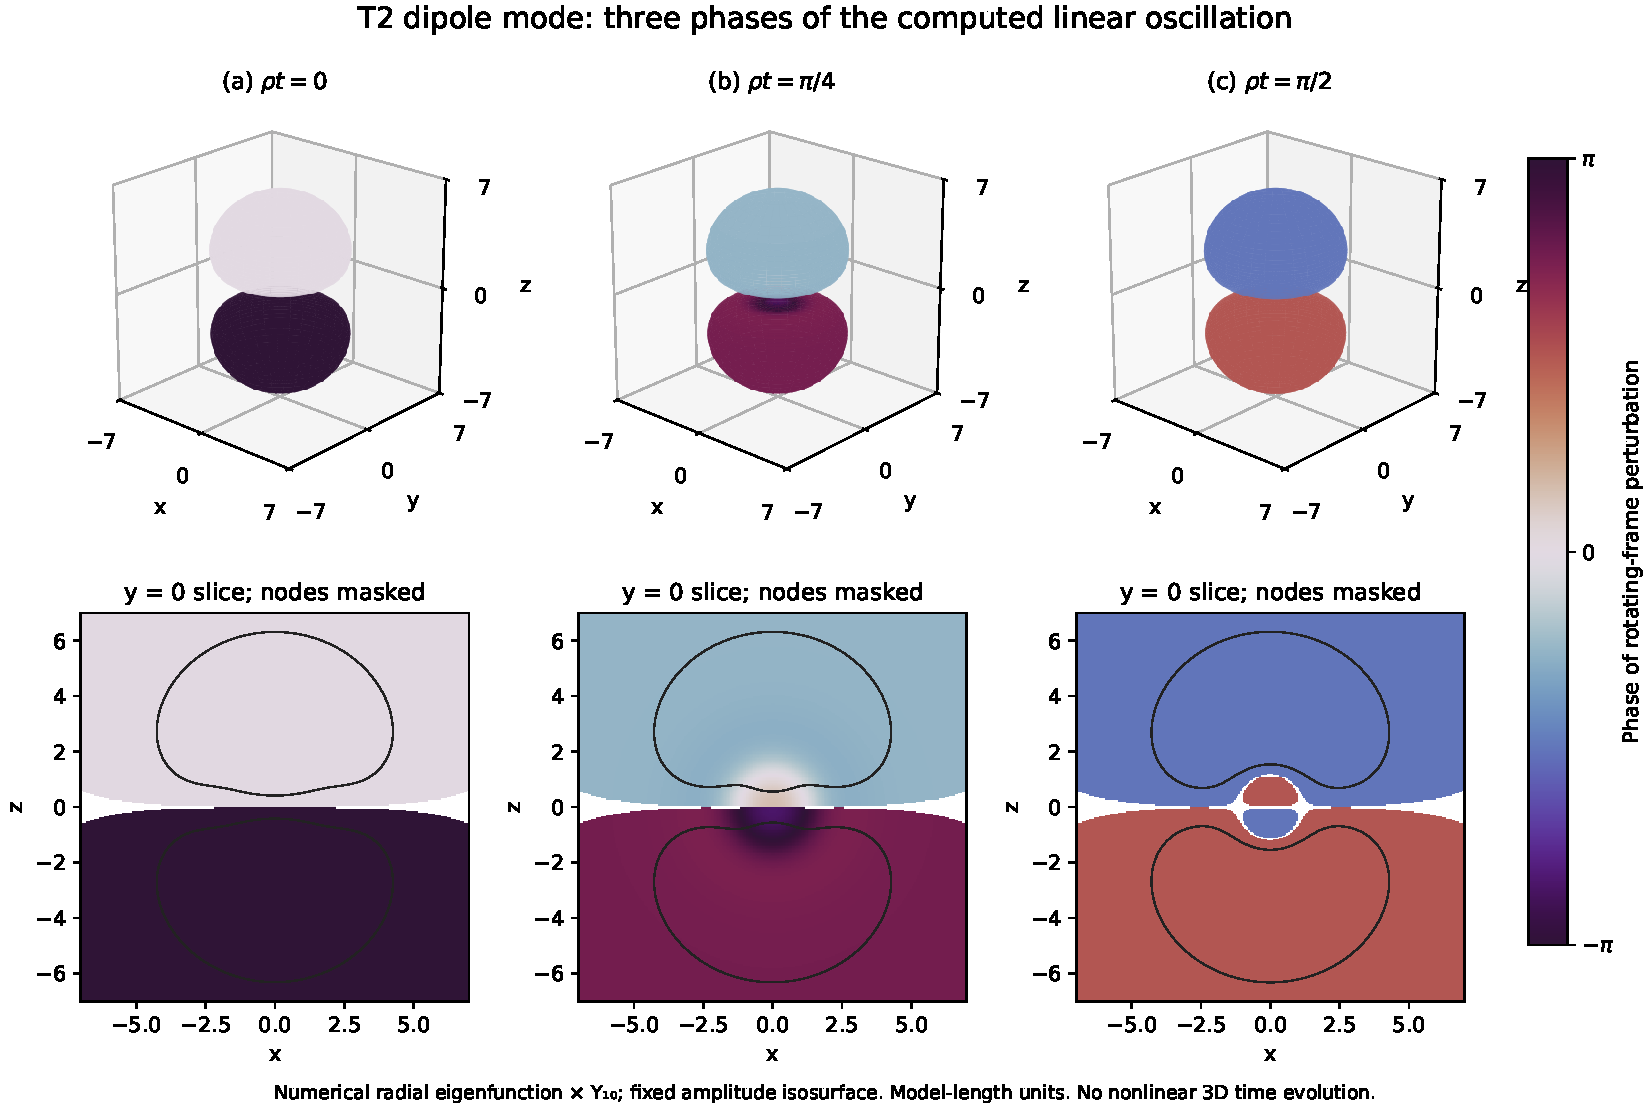
\includegraphics[width=.88\linewidth]{dipole-phases.pdf}
\caption{Numerical reconstruction near the enclosed dipole mode C2, with
angular factor $Y_{10}=\sqrt{3/(4\pi)}z/r$. Top: three phases of the
linear perturbation; bottom: $y=0$ sections with phase masked below
$1.5\%$ of the common displayed maximum. The time factors are the two
linear sidebands, not a nonlinear evolution. The stored visualization's
historical label is mapped to C2 in the archive figure inventory.}
\label{fig:core-dipole}
\end{figure}
\section{Computer-assisted existence results}
\label{sec:certified-existence}

We distinguish the three computer-assisted existence results below from
the numerically observed ladder. The proof establishes a localized mode
at a parameter pair inside each specified box. It does not certify every
observed radiation minimum, an infinite ladder, or a nonlinear
nonradiating solution.

\subsection{Model and precise statement}
\label{sec:proof-model}
Consider the complex Klein--Gordon equation in three spatial dimensions,
\begin{equation}
 \partial_t^2\phi-\Delta\phi+U'(|\phi|^2)\phi=0,
 \qquad U(S)=S-S^2+\tfrac12 S^3.
 \label{eq:proof-kg}
\end{equation}
A stationary Q-ball has the form $\phi_0=e^{i\omega t}f(r)$, where
\begin{equation}
 f''+\frac{2}{r}f'=(1-\omega^2)f-2f^3+\tfrac32 f^5,
 \qquad f(0)=a,\quad f'(0)=0.
 \label{eq:proof-profile}
\end{equation}
We use a real orthonormal basis $Y_{\ell m}$ of spherical harmonics and
write a linear perturbation as
\begin{equation}
 \delta\phi=e^{i\omega t}
 \left[\frac{A(r)}{r}e^{i\rho t}
       +\frac{B(r)}{r}e^{-i\rho t}\right]Y_{\ell m}.
 \label{eq:proof-mode}
\end{equation}
In a complex harmonic basis the second sideband instead contains
$Y_{\ell m}^*$. With $S=f^2$, substitution in the linearization of
\eqref{eq:proof-kg} gives
\begin{equation}
 \begin{aligned}
 A''&=\left[1-4S+\tfrac92 S^2-(\omega+\rho)^2
                  +\frac{\ell(\ell+1)}{r^2}\right]A+CB,\\
 B''&=\left[1-4S+\tfrac92 S^2-(\omega-\rho)^2
                  +\frac{\ell(\ell+1)}{r^2}\right]B+CA,
 \qquad C=-2S+3S^2.
 \end{aligned}
 \label{eq:proof-radial-system}
\end{equation}
Regularity requires $A,B=O(r^{\ell+1})$. Define
\begin{equation}
 \kappa_0=\sqrt{1-\omega^2},\qquad
 k=\sqrt{(\omega+\rho)^2-1},\qquad
 \kappa_c=\sqrt{1-(\omega-\rho)^2}.
 \label{eq:proof-channel-numbers}
\end{equation}

\noindent\textbf{Computer-assisted existence statement.}
For each row of Table~\ref{tab:proof-cases}, the corresponding certificate
encloses a quadruple $(a_*,c_*,\rho_*,\omega_*)$ with $c_*>0$ such that
\eqref{eq:proof-profile} has a positive global solution satisfying
$r e^{\kappa_0r}f(r)\to c_*$, and
\eqref{eq:proof-radial-system} has a nonzero real solution regular at the
origin with
\begin{equation}
 |A(r)|+|B(r)|\leq K_J e^{-\kappa_c r}\quad(r\geq L),
 \qquad e^{\kappa_c r}B(r)\longrightarrow1.
 \label{eq:proof-decay}
\end{equation}
The resulting spatial fields in \eqref{eq:proof-mode} are smooth and
exponentially localized. The certification is
conditional on the correctness of the stated interval-arithmetic
implementation and its underlying arithmetic libraries.

\begin{table}[htbp]
\centering
\small
\begin{tabular}{ccll}
\hline
Case & $\ell$ & Enclosure of $\omega_*^2$ & Enclosure of $\rho_*$ \\
\hline
C0 & 0 & $0.797676787111865191750\pm4.8\,10^{-22}$
       & $1.744617544837398735781\pm6.8\,10^{-22}$ \\
C1 & 0 & $0.6851289044582160933\pm2.5\,10^{-20}$
       & $1.6903565973281434568\pm4.7\,10^{-20}$ \\
C2 & 1 & $0.7544960137826372331\pm7.8\,10^{-20}$
       & $1.826342030181069956\pm3.0\,10^{-19}$ \\
\hline
\end{tabular}
\caption{The three certified parameter boxes, displayed as outward-rounded
decimal enclosures. The proof uses the full exact dyadic boxes in
$(a,c,\rho,\omega)$, not these two-coordinate summaries.
Their numerical ladder
assignments are $(\ell,n)=(0,1),(0,2),(1,1)$; the labels $n$ are not
separately certified nodal counts.}
\label{tab:proof-cases}
\end{table}

For the enclosed parameter pair and its fixed radial angular channel, every
solution of \eqref{eq:proof-radial-system} that is square integrable on
$[L,\infty)$ is a scalar multiple of the constructed solution. This is
\emph{geometric radial simplicity}. It neither establishes algebraic
simplicity of a dynamical generator nor excludes Jordan chains. For C2,
the three-dimensional $\ell=1$ angular multiplet remains degenerate.
The translation mode at $\rho=0$ does not belong to the fixed nonzero
frequency considered here.

The term \emph{embedded} is used operationally: $k^2>0$ and
$\kappa_c^2>0$, so a free asymptotic channel is open, while the constructed
mode is exponentially localized and has no oscillatory radiation tail.
We do not identify the essential spectrum of a fully specified operator
pencil in this proof. The perturbation is periodic after removing
$e^{i\omega t}$; the two laboratory frequencies are $\omega\pm\rho$,
with no claim about their rational commensurability.

\subsection{Infinite-domain construction and inclusion}
\label{sec:proof-tails}
The matching radius $L$ joins an interval-integrated core to an analytic
infinite exterior. The potential and its coupling are retained beyond
$L$. Appendix~\ref{supp:proof-lemmas} gives the complete
analytic lemmas used below, including the origin start and the error
bounds for every Taylor step.

For the profile, $\widetilde u=r e^{\kappa_0r}f$ satisfies
\begin{equation}
 \widetilde u(r)=c+\int_r^\infty
 \frac{1-e^{-2\kappa_0(s-r)}}{2\kappa_0}
 \left(-2f(s)^2+\tfrac32f(s)^4\right)\widetilde u(s)\,\dd s.
 \label{eq:proof-profile-volterra}
\end{equation}
The certified exterior constants give a uniform contraction in a positive
ball about $c$. For the mode, the free open and closed Green kernels
produce a Volterra equation with integrable coefficients. Ordered
iteration has factorial error majorants, and yields a normalized
exponentially decaying Jost solution. The $\ell=1$ construction retains
the exact Riccati functions and the centrifugal term. These constructions
supply continuous corrections to both the profile Cauchy data and the
mode Cauchy data at $L$, uniformly on the parameter box.

\subsection{Finite-dimensional certificate}
\label{sec:proof-krawczyk}
Let $z=(a,c,\rho,\omega)$. The four-component matching map is
$H=H_0+E$. Its first two components match profile value and derivative;
the last two are scaled Wronski forms
$W(\Psi,R_i)=\Psi\cdot R_i'-\Psi'\cdot R_i$, where $R_1,R_2$ are
the two regular origin solutions. The nominal map $H_0$ uses the free
Jost data and $E$ bounds the infinite-tail correction.
For $\ell=0$, these pairings equal the origin values of $\Psi$.
For $\ell=1$, the regular behaviors $r^2e_i$ pair with singular
behaviors $r^{-1}e_i/3$ to give $\delta_{ij}$. Thus their joint vanishing
is precisely regularity of the Jost solution at the origin.

The core integration encloses $H_0(z_0)$ and $DH_0(Z)$ using complex
analytic a priori bounds and Taylor remainders. At the origin, the
profile integral equation has weight mass $r^2/6$; for
$A=r^2\alpha$, $B=r^2\beta$ the $\ell=1$ weight mass is $r^2/10$.
Parameter derivatives are integrated as part of the same enclosed
system. All step choices and preconditioners become exact dyadic input;
acceptance uses directed arithmetic.

Write $Z=z_0+[-\delta,\delta]$, let $D$ enclose $DH_0(Z)$, and let
$|E_i|\leq\epsilon_i$ throughout $Z$. A fixed dyadic matrix $Y$ gives
\begin{equation}
 \begin{split}
 z_0-YH_0(z_0)+(I-YD)[-\delta,\delta]
       +|Y|[-\epsilon,\epsilon]&\subset\operatorname{int}Z,\\
 \max_i\sum_j |I-YD|_{ij}\frac{\delta_j}{\delta_i}&<1.
 \end{split}
 \label{eq:proof-krawczyk-inclusion}
\end{equation}
The first inclusion makes $z\mapsto z-YH(z)$ a continuous self-map of
$Z$. Brouwer gives a fixed point; the weighted matrix inequality makes
$Y$ invertible, so $H(z_*)=0$. This proof requires continuity, but no
derivative bound, for $E$ and does not assert uniqueness of $z_*$.
Positive core enclosures, a minimum-principle argument on the remaining
finite interval, and the positive exterior fixed point establish $f>0$.
Finally $2\kappa_0>\kappa_c$ permits two bounded oscillatory comparison
solutions at infinity. Their nonzero mutual Wronskian and the
four-dimensional symplectic Cauchy-data space imply that every
square-integrable solution is a multiple of the decaying Jost solution.
Appendix~\ref{supp:simplicity} supplies this simplicity proof explicitly.

\subsection{Certificate contents and verification scope}
\label{sec:proof-verification-limits}
The defining certificates use $L=40$ for C0, $L=32$ for C1, and $L=36$
for C2, with 256-bit ball arithmetic. The preserved historical records
identify these three JSON certificates by case, filename and SHA-256
checksum. A distribution copy with redacted execution metadata is a
derivative: the archive manifest lists its checksum separately from the
historical checksum, while retaining the numerical fields. The full
dyadic boxes, channel bounds, tail constants,
inclusion results and integration-step records are the proof inputs.
The fresh primary-certificate reproduction uses the preserved historical
proof-code bytes. The distribution provides separately hashed code
derivatives with redacted comments and one metadata string in the unused
starting-value-search mode; \texttt{CODE-HASH-MAP.tsv} records their
correspondence. These changes leave the certificate execution path unchanged.
A filename recorded by an old driver is resolved through its recorded
hash, rather than assumed to identify a later file with the same name.

Additional runs use larger matching radii and 320-bit arithmetic. C2's
original repeat at $L=40$ failed the inclusion test; a subsequent run
with an enlarged $c$-radius passed after reevaluating all bounds on that
box. This is an adaptive additional certificate. The C2 existence claim
rests on the first successful certificate alone.

For C0, $2\kappa_0>\kappa_c$ was recorded and separately checked but
was absent from the historical aggregate success flag. This documented
flag omission is retained. For preprint 0.51 a separate ball-arithmetic
check reconstructs the exact dyadic parameter box from the reproduced
C0 receipt and verifies $2\kappa_0-\kappa_c>0$ throughout that box,
together with $\rho>\omega$. It binds the checked receipt and the checker
by their checksums; neither the historical driver nor its success flag
is amended.
The C1/C2 drivers include the inequality explicitly. Repeated runs and
code review use the same implementation and do not supply an independent
second implementation; no alternative interval library and no formal
proof assistant were used. Correctness of Python--FLINT, Arb/Acb and the
recorded execution remains part of the computational trust base
(Section~\ref{sec:discussion}).

The arithmetic uses midpoint--radius enclosures
\cite{Johansson2017Arb,PythonFlintDocs,FlintSoftware}; the finite-dimensional
inclusion is of Krawczyk type \cite{Krawczyk1969}, with the explicit
Brouwer argument above for the continuous tail correction. The three
linear existence results leave background stability, algebraic spectral
simplicity and certification of the full empirical ladder open.

\section{Numerical radial sequence}\label{sec:sequence}
A width minimum is a numerical candidate; a resolved winding of a
specified two-component matching map adds numerical evidence; an
interval enclosure with analytic tails establishes infinite-domain
existence. Table~\ref{tab:ladder} keeps these levels separate.
The winding concept has a photonic BIC precedent~\cite{Zhen2014}; here
it is applied to a matching map in parameter space, without transferring
the photonic symmetry-based robustness theorem.
For indices 5--18, the matching map tests whether the exterior decaying
Jost solution is regular at the origin; the locations are numerical
zeros of this map. In the truncated exterior model this solution has
zero open-channel value and derivative at the outer radius and a
decaying closed-channel component. No reflecting-box eigenvalue
condition is imposed. The earlier records of indices 3--5 and the
linewidth rows 11--14 use outgoing Hankel conditions.
Increasing the outer radius by 20 and 40 units moved the locations of
indices 3, 8 and 13 by at most $1.3\times10^{-10}$ in $\omega^2$ and that
of index 18 by about $1.5\times10^{-6}$, within its estimated roundoff
level of $4.6\times10^{-6}$. This shows insensitivity to the truncation
radius, not an exact zero width.
The refined matching calculation for indices $6$--$10$ used radial
steps $0.04$ and $0.02$. Its locations interpolate parameter samples
separated by $2.5\times10^{-4}$. For indices $7$--$10$, the small
inter-grid difference ($2.3\times10^{-8}$ or less) is not a validated location error.
The reported interpolation uncertainty is a few $10^{-6}$.
For indices $11$--$14$, the archived linewidth reconstruction used signs
chosen to match neighboring slopes; index $5$ had a sign change without
a resolved winding. For this revision, indices $5$ and $11$--$14$ were
recomputed with the unchanged matching program and parameters of the
index-$15$--$18$ calculation. The rung acceptance thresholds were
retained from that calculation: one sign change of the matching error
among five starting rows, root brackets of at most $10^{-9}$ on radial
steps $0.04$ and $0.02$ with locations agreeing to $10^{-6}$, and a
rectangle crossing count $\pm1$ with alternating signs. Before this run
we additionally required a sampled phase winding equal to the crossing
count with every phase jump below $0.4$ radians. The computational time
budget was increased. The control reproduces the earlier $h=0.04$
index-$15$ root to $5\times10^{-13}$; for index $5$, the prespecified
alternation check uses index $4$. All five rungs met these conditions:
crossing counts $-1,+1,-1,+1$ for indices $11$--$14$ (and $-1$
for index $15$), $-1$ for index $5$, maximum phase jumps $0.28$--$0.30$
radians, final brackets $\le8.7\times10^{-10}$ and grid differences
$\le3.2\times10^{-8}$. The new locations differ from the earlier
estimates by $2.4\times10^{-6}$ (index $5$), $1.6\times10^{-6}$ (index
$11$) and at most $1.9\times10^{-7}$ (indices $12$--$14$). With these
locations and the subsequent index-$15$ location, the inverse-detuning
steps for indices $11$--$15$ are $2.3036$, $2.3045$, $2.3053$ and
$2.3059$. This raises the five rows to resolved numerical windings; it
is numerical evidence in the truncated model, not a certificate.

\begin{table}[htbp]\centering\small
\caption{Radial candidates at $\beta=1/2$. Displayed numerical digits
are not interval enclosures. Certificates C0/C1 are given in
Section~\ref{sec:certified-existence}; the remaining entries are finite-domain
numerical evidence. The last three error estimates are empirical.
``(0.53)'' marks rows raised by the matching calculation of this
revision.}
\label{tab:ladder}
\begin{tabular}{rll}\toprule
$n$&$\omega^2$&Evidence\\\midrule
1&$0.797676787\ldots$&Existence enclosure C0\\
2&$0.685128904\ldots$&Existence enclosure C1\\
3&$\sim0.631450$&Resolved numerical winding\\
4&$\sim0.601421$&Resolved numerical winding\\
5&$\sim0.5824198$&Resolved numerical winding (0.53)\\
6&$\sim0.569360$&Resolved numerical winding\\
7&$\sim0.559848$&Resolved numerical winding\\
8&$\sim0.552619$&Resolved numerical winding\\
9&$\sim0.546940$&Resolved numerical winding\\
10&$\sim0.542364$&Resolved numerical winding\\
11&$\sim0.5386009$&Resolved numerical winding (0.53)\\
12&$\sim0.5354487$&Resolved numerical winding (0.53)\\
13&$\sim0.5327715$&Resolved numerical winding (0.53)\\
14&$\sim0.5304696$&Resolved numerical winding (0.53)\\
15&$\sim0.52846934$&Subsequent resolved winding\\
16&$0.52671542\pm2\times10^{-7}$&Resolved winding, final bracket rule failed\\
17&$0.52516277\pm1.3\times10^{-6}$&Resolved winding, final bracket rule failed\\
18&$0.5237875\pm4\times10^{-6}$&Crossing count $+1$; phase unresolved\\\bottomrule
\end{tabular}
\end{table}

The subsequent calculation reproduced index $15$ near $0.5284693357$.
For $16$ and $17$, resolved numerical windings are $+1$ and $-1$.
For $18$, the crossing count and sampled phase winding both give $+1$,
but the maximum phase jump $0.585$ radians fails the resolution rule.
All three miss the prescribed final-bracket acceptance criterion; the
empirical errors include roundoff sensitivity. This unsuccessful
combined acceptance rule is retained, even where individual diagnostics
are informative. There is no certificate or completeness result for
these additional candidates.

\begin{figure}[htbp]\centering
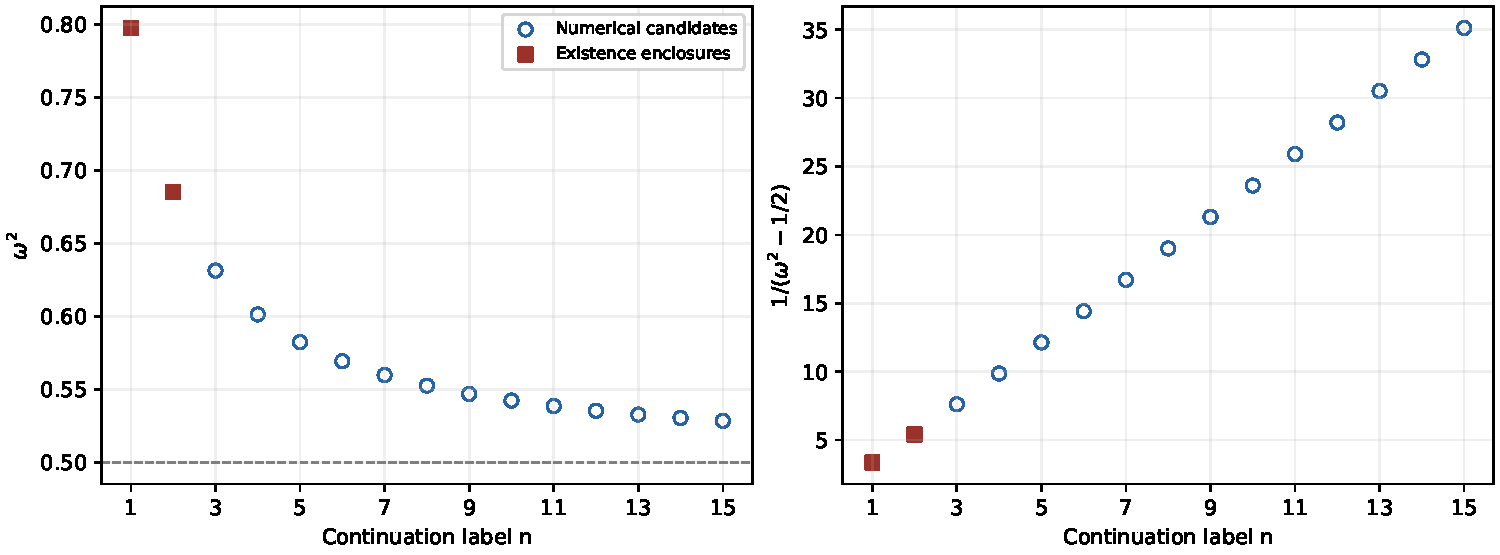
\includegraphics[width=.9\linewidth]{ladder.pdf}
\caption{Archived radial locations through $n=15$ and their inverse
detunings $1/(\omega^2-1/2)$. Filled symbols mark C0/C1. The plot retains
its original fifteen-point dataset, including the earlier rounded
index-$15$ estimate and the earlier locations of indices $5$ and
$11$--$14$; Table~\ref{tab:ladder} records the subsequent $15$--$18$
calculation and the recomputed indices $5$ and $11$--$14$ explicitly. The supplementary source inventory
binds the figure to its data. No new fit or extrapolated points are added.}
\label{fig:ladder}
\end{figure}

\paragraph{Prediction history.}\label{sec:predictions}
A sequential extrapolation was updated after each group of targets.
A separate four-parameter thin-wall fit used indices $5,7,8,9$;
its author reported separation from later target values, which were
already known to the coordination team. The frozen file of
30 September 2026, 08:33:26 CEST, and its SHA256 binding are included in
the supplementary source inventory. This is a documented calibrated
extrapolation, not global preregistration. The five later comparisons
passed their respective diagnostic windows, but showed a systematic
thin-wall offset of about $2\times10^{-5}$, comparable to those windows.
The unfitted planar comparison below therefore carries the mechanistic
interpretation; the forecast history does not establish zero linewidth.

\section{Thin-wall phase matching and a planar transmission zero}\label{sec:thinwall}
Put $\epsilon=\omega^2-\omega_c^2$ and $S_c=1/(2\beta)$.
The leading thin-wall profile and radius in three dimensions are
\begin{equation}\label{eq:thinwall}
R_{\mathrm{tw}}\simeq\frac{1}{2\sqrt\beta\,\epsilon},\qquad
f^2(r)\simeq\frac{S_c}{1+\exp[(r-R_{\mathrm{tw}})/\sqrt\beta]}.
\end{equation}
These are asymptotic approximations, not substitutes for the certified
profiles. The leading radius relation is established prior work: with
$\Delta=m_\phi^2-\omega_0^2$, Heeck et al. use
$\kappa^2=(\omega^2-\omega_0^2)/\Delta$ and
$R^*=\sqrt\Delta R$, and obtain $R^*\simeq1/\kappa^2$
in their Eq.~(40)~\cite{Heeck2021}.
Here $\Delta=1/(4\beta)$, which gives the radius in
Eq.~\eqref{eq:thinwall}. Their inflection-point radius and our
half-density radius need not have identical subleading coefficients.
Their Eq.~(58) gives
$R^*=\kappa^{-2}+\tfrac14-\tfrac{5}{16}\kappa^2+O(\kappa^4)$;
these terms require a radius-convention conversion before comparison
with the present half-density radius~\cite{Heeck2021}.
Diagonalizing the constant interior channel matrix gives the
propagating interior wavenumber
\begin{equation}\label{eq:interior}
k_{\mathrm{in}}^2=\omega^2+\rho^2-D_c+
 \sqrt{4\omega^2\rho^2+C_c^2},\qquad
D_c=1+\frac1{4\beta},\quad C_c=\frac1{2\beta}.
\end{equation}
At the stated interior amplitude, this is the same dispersion branch as
Eq.~(101) of Zhang, Zhou, and Zhu~\cite{ZhangZhouZhu2025}; the interior
wavenumber is an established ingredient, not a new result here.
A regular interior standing wave reaches the wall with phase
$\Psi=k_{\mathrm{in}}R_{\mathrm{tw}}$. The bare closed-channel wall approximation
supplies a localized state, while matching it to the open interior
wave permits a sign-changing radiation amplitude. A useful leading
parametrization is
\begin{equation}\label{eq:phase}
k_{\mathrm{in}}(\omega_n,\rho_n)R_{\mathrm{tw}}(\omega_n)
 \simeq\pi[n+\theta(\epsilon_n)],\qquad
\rho_n\simeq\omega_n+c(\epsilon_n).
\end{equation}
The radius and interior dispersion follow from the model approximations;
the wall phase $\theta$ and dressed level shift contained in $c$ remain
calibrated. A separate coupled planar-wall calculation now supplies a
numerical transmission zero, but does not determine both finite-curvature
functions independently. Consequently, agreement of the calibrated
phase rule with the sequence is not a parameter-free prediction.

For $\beta=1/2$ and $\omega^2=1/2$, the exact planar profile is
$S(x)=[1+\exp(\sqrt2 x)]^{-1}$. Solving the two-channel scattering
problem, with one open and one evanescent channel on each side, gives
\begin{equation}\label{eq:planarzero}
\rho_z\simeq1.52414976213,\qquad
k_{\mathrm{in}}(\rho_z)\simeq1.92332459129.
\end{equation}
An independently implemented Numerov boundary-value calculation confirmed
this zero before reading the comparison calculation. It used a continuously
phase-normalized transmission amplitude, actual complex-transmission
residuals, flux and reciprocity controls, and separate mesh and boundary
refinements. A conservative empirical frequency uncertainty is $10^{-9}$;
this is not a certified enclosure. Two finite frequency scans found no
additional zero, but do not prove uniqueness throughout the open-channel
window. The planar scattering state has an incident and reflected wave;
it is not itself a square-integrable embedded mode.

If $k_{\mathrm{in}}\to k_\infty>0$ and the wall phase has a finite limit,
Equation~\eqref{eq:phase} predicts, within the approximation,
\begin{equation}\label{eq:spacing}
\epsilon_n\sim\frac1{b_\infty n},\qquad
b_\infty=\frac{2\sqrt\beta\,\pi}{k_\infty}.
\end{equation}
From the historical rounded locations $0.535449$, $0.532772$,
$0.530470$, $0.528469$, the inverse-detuning steps for indices 12--15
are approximately 2.3043, 2.3053 and 2.3068;
these descriptive values do not specify accuracy beyond the input locations.
The matching locations added in this revision (Section~\ref{sec:sequence})
give $2.3045$, $2.3053$ and $2.3059$ for the same three steps.
The calibrated model gives 2.298, while its bare
wall-state estimate gives 2.334. Substituting the independently computed
planar zero into Equation~\eqref{eq:spacing} instead gives
$b_\infty^{\mathrm{wall}}\simeq2.31000162857$, with a conservative empirical
numerical uncertainty of $2\times10^{-9}$. This wall-based candidate was not
fitted to ladder locations. Identifying it with the actual radial limiting
step still requires a controlled curvature and phase-matching limit.
This supports a useful spacing description;
it does not prove existence of infinitely many localized modes or identify
an exact limiting constant. The phase model also motivates alternating
signs of a matching Jacobian and quadratic linewidth minima, but neither
property independently replaces a tail-controlled existence proof.

The open part of this description can be stated precisely.
\begin{conjecture}[radial ladder and limiting spacing]\label{conj:ladder}
Let $\beta=1/2$ and $\ell=0$. There is an index $n_0$ such that for
every $n\ge n_0$ there is a parameter pair $(\omega_n,\rho_n)$ with
$\omega_c<\omega_n<1$ and $1-\omega_n<\rho_n<1+\omega_n$ at which
Eq.~\eqref{eq:proof-profile} has a positive global solution with
$f(r)\to0$ and Eq.~\eqref{eq:proof-radial-system} has a nonzero real
solution regular at the origin that obeys the decay
bound~\eqref{eq:proof-decay} for some $K_J$ and $L$, which may depend
on $n$. These pairs can be chosen such that $\epsilon_n=\omega_n^2-1/2$
decreases strictly, $\epsilon_n\to0$, $\rho_n\to\rho_z$, and
\begin{equation*}
\epsilon_{n+1}^{-1}-\epsilon_n^{-1}\longrightarrow
b_\infty^{\mathrm{wall}}=\frac{2\sqrt\beta\,\pi}{k_{\mathrm{in}}(\rho_z)}
\simeq2.3100 .
\end{equation*}
Here $\rho_z$ denotes the conjectured simple zero of the exact planar
transmission amplitude near the numerical value of
Eq.~\eqref{eq:planarzero}, and $k_{\mathrm{in}}$ is evaluated at
$\omega=\omega_c$.
\end{conjecture}
The evidence for Conjecture~\ref{conj:ladder} is numerical and
heuristic: certificates for $n=1,2$; finite-domain candidates through
$n=18$ whose inverse-detuning steps rise slowly, from $2.3036$ to
$2.3059$ between indices $11$ and $15$ in the matching locations of
Section~\ref{sec:sequence}; and the uncertified planar transmission
zero. Three ingredients of a proof are missing: (i)~an enclosure of the
planar zero $\rho_z$ together with a nondegeneracy (transversality)
condition; (ii)~estimates, uniform as $\epsilon\to0$, that control the
difference between the rescaled curved-wall matching map and its planar
limit, including the deviation of the profile from the planar kink and
the $1/r$ and centrifugal terms; and (iii)~a quantization estimate
controlling successive phase increments, sufficient to establish
convergence of the inverse-detuning gaps, together with a degree or
fixed-point argument that converts (i) and (ii) into one localized mode
per index.
None of them is attempted here. The finite steps are compatible with
convergence to $2.3100$ but do not demonstrate it; for $\beta=1$ the
reported steps ($2.5964$ to $2.6038$, below) remain about $0.6$--$0.9\,\%$
below their planar candidate $2.6186$.
The inverse-first-power scaling follows from the calibrated model, not
from an independently established asymptotic exponent. Exploratory free
power fits yielded exponents between $-0.76$ and $-0.88$; the reciprocal
fit improved the comparison metric only by factors of approximately
$1.2$--$2$, below the originally sought factor of ten. Finite-data agreement
therefore does not establish an exact asymptotic law.

A local numerical check also supports a planar transmission cancellation
for the modified potential $U(S)=S-S^2+S^3$ at
$\omega_{\min}=\sqrt{3}/2$. An independent Numerov implementation,
with the candidate frequency already known, gives
$\rho_z\simeq1.77345307180$ and $k_{\mathrm{in}}\simeq2.3994321234$.
The last grid change, $h=0.04$ to $0.02$, shifts $\rho_z$ by
$1.64\times10^{-10}$, while increasing the half-domain from $32$ to $40$
at the finest spacing changes it by $4.2\times10^{-14}$; these are
empirical sensitivities, not certified bounds. The corresponding thin-wall
spacing candidate is $2\pi/k_{\mathrm{in}}\simeq2.618613482$. This known-target
local replication neither counts all planar zeros nor establishes the
radial ladder limit for the modified potential.

The corresponding radial calculation is also available. Its last
previously reported inverse-detuning step was $2.596420$, about $0.9\%$
below the planar candidate. A subsequent search gave the following
finite-domain numerical locations; $k$ continues that study's local
index and is not a certified node count:
\begin{center}\small
\begin{tabular}{rlll}\toprule
$k$&$\omega^2$&$1/(\omega^2-3/4)$&Resolved winding\\\midrule
0&$0.778585440$&$34.98284$&$-1$\\
$-1$&$0.776606628$&$37.58462$&$+1$\\
$-2$&$0.774882776$&$40.18844$&$-1$\\\bottomrule
\end{tabular}\end{center}
The reported empirical uncertainties are about $2\times10^{-8}$ in
$\omega^2$ and $3\times10^{-5}$ in inverse detuning. These later
increments are approximately $2.6018$ and $2.6038$; convergence to the
planar value remains a conjectural interpretation. A frozen
absolute-location formula truncated after the $O(1)$ term failed its
combined test: inverse-detuning errors for this potential were
$0.23$--$0.26$, outside the preassigned $0.10$ window; an extrapolation
of the preceding radial locations was more accurate for both potentials.
This failure concerns the finite-order absolute-location formula,
not a proof or disproof of the leading wall spacing.

\section{Nonlinear sources and the limits of linear trapping}
\label{nl:section}

A localized eigenmode of the linearized equation need not remain
radiationless at finite amplitude. We distinguish an exact source
calculation, the kinematic opening of radiation channels, and a nonzero
outgoing response. Existing nonlinear evidence for radial location C0
is described below; it is not transferred to the additional modes C1
and C2 without evaluating their own sources.

\subsection{Quadratic expansion}
\label{nl:expansion}
We use the complex nonlinear Klein--Gordon equation
\begin{equation}
 \phi_{tt}-\Delta\phi+U'(|\phi|^2)\phi=0,
 \qquad U(S)=S-S^2+\tfrac12 S^3,
 \qquad \phi=e^{i\omega t}(f+z),
 \label{nl:model}
\end{equation}
where the real background satisfies
$-\Delta f-\omega^2f+U'(f^2)f=0$. Setting $s=f^2$, the linear operator is
\begin{equation}
 \mathcal Lz=z_{tt}+2i\omega z_t-\Delta z
 +[U'(s)+sU''(s)-\omega^2]z+sU''(s)\overline z.
 \label{nl:linear}
\end{equation}
The quadratic term in the equation's left-hand side is exactly
\begin{align}
 G_2[z]&=fU''(s)(z^2+2|z|^2)
       +\tfrac12 f^3U'''(s)(z+\overline z)^2 \nonumber\\
       &=\mathcal A z^2+2\mathcal A|z|^2+\mathcal C\overline z^{\,2},
 &\mathcal A&=f\left(-2+\tfrac92f^2\right),
 \qquad \mathcal C=\tfrac32f^3.
 \label{nl:quadratic}
\end{align}
Consequently $z=\epsilon z_1+\epsilon^2z_2+\cdots$ gives
$\mathcal Lz_1=0$ and $\mathcal Lz_2=-G_2[z_1]$. In particular, the
forcing has the opposite sign to the Taylor term in
Eq.~\eqref{nl:quadratic}.

For a real spherical harmonic $Y$ and real radial functions $a,b$, write
\begin{equation}
 z_1=Y\bigl(ae^{i\rho t}+be^{-i\rho t}\bigr).
\end{equation}
Then
\begin{align}
 G_2[z_1]&=Y^2\bigl(Q_+e^{2i\rho t}+Q_0+Q_-e^{-2i\rho t}\bigr),\\
 Q_+&=\mathcal A(a^2+2ab)+\mathcal Cb^2,\qquad
 Q_-=\mathcal A(b^2+2ab)+\mathcal Ca^2,\\
 Q_0&=2\mathcal A(a^2+b^2)+2(\mathcal A+\mathcal C)ab.
 \label{nl:coefficients}
\end{align}
These expressions introduce rotating-frame frequencies $0,\pm2\rho$,
or laboratory frequencies $\omega,\omega\pm2\rho$. The zero-frequency
term is static only in the rotating frame.

\subsection{Angular selection and forced channel problems}
\label{nl:selection}
For C1, the radial $l=0$ mode, $Y=Y_{00}$ and
$Y_{00}^2=Y_{00}/\sqrt{4\pi}$, so only $L=0$ occurs at this order.
For C2, choose a real normalized $l=1$ harmonic. After a spatial rotation
it equals $Y_{10}$, and
\begin{equation}
 Y_{10}^2=\frac{Y_{00}}{\sqrt{4\pi}}
          +\frac{Y_{20}}{\sqrt{5\pi}}.
 \label{nl:angular}
\end{equation}
Thus each of the three temporal source coefficients can drive $L=0$
and $L=2$; the antisymmetric $L=1$ product is absent. A different real
orientation rotates the quadrupole within the $L=2$ multiplet. This
standing real mode must not be confused with a rotating complex
$Y_{11}/\overline{Y}_{11}$ block: the latter has
$Y_{11}^2=\sqrt{3/(10\pi)}Y_{22}$ for its corresponding oscillatory product.

Let $c_L$ denote the coefficient in the relevant angular product and
$D_L=-\partial_r^2-2r^{-1}\partial_r+L(L+1)r^{-2}$. For the oscillatory
response $h_{+,L}e^{2i\rho t}+h_{-,L}e^{-2i\rho t}$ one must solve
the coupled system
\begin{equation}
 \begin{pmatrix}
 D_L+U'+sU''-(\omega+2\rho)^2&sU''\\
 sU''&D_L+U'+sU''-(\omega-2\rho)^2
 \end{pmatrix}
 \begin{pmatrix}h_{+,L}\\\overline{h}_{-,L}\end{pmatrix}
 =-c_L\begin{pmatrix}Q_+\\Q_-\end{pmatrix}.
 \label{nl:forced}
\end{equation}
Here $U',U''$ are evaluated at $s$; the conjugated second unknown matters
when imposing outgoing conditions. The real static correction obeys
$[D_L+U'+2sU''-\omega^2]h_{0,L}=-c_LQ_0$.
Gauge and charge constraints must also be fixed in constructing a
nonlinear continuation.

Both C1 and C2 have $|\omega|<1$ and $|\omega\pm2\rho|>1$.
For C2, the latter frequencies are approximately $4.52130$ and $-2.78407$.
The second harmonics are therefore open in the mass-one vacuum, whereas
the rotating-static correction is closed. The centrifugal term does
not change the asymptotic mass threshold. With the convention
$e^{iEt}$, an outgoing wave has radial phase
$e^{-i\operatorname{sgn}(E)\sqrt{E^2-1}\,r}$; a negative $E$ does not
mean negative outward energy transport.

An open channel and a nonzero local source do not establish radiation:
the outgoing source overlap can vanish. A localized continuation without
incoming radiation requires both open amplitudes to vanish in every
allowed $L$ block of Eq.~\eqref{nl:forced}. The C1 response remains open;
an approximate-input C2 calculation is reported below. A nonzero such amplitude would obstruct
a regular localized perturbative continuation with the specified leading
mode, but would not exclude all other nonlinear states. Frequency shifts
of order $\epsilon^2$ do not automatically cancel the second harmonic:
the carrier shift contributes a static background correction at this
order, while a shift of $\rho$ first acts on $\epsilon z_1$ at order
$\epsilon^3$.

\subsection{Complex dipole polarization and a conditional obstruction}
\label{nl:polarization}
The threefold dipole degeneracy allows more than rotations of a real
standing mode. Let $Y_i(\boldsymbol n)=\sqrt{3/(4\pi)}n_i$ be real
orthonormal Cartesian dipole harmonics and write
$A(\boldsymbol n)=\sum_i p_iY_i(\boldsymbol n)$, with
$\boldsymbol p\in\mathbb C^3$. For the same real radial eigenmode as above,
the allowed tangent has the linked sidebands
$z_1=a(r)A e^{i\rho t}+b(r)\overline A e^{-i\rho t}$.
This does not allow independently chosen polarizations of the two
sidebands or a mixture of distinct radial modes.

Set $\nu=\boldsymbol p^\dagger\boldsymbol p$ and
$\chi=\boldsymbol p^T\boldsymbol p$. The oscillatory quadratic forcing
is proportional to $A^2$, rather than $|A|^2$. Its orthogonal angular
projections satisfy the exact identities
\begin{equation}
 \|P_0(A^2)\|_{L^2(S^2)}^2=\frac{|\chi|^2}{4\pi},\qquad
 \|P_2(A^2)\|_{L^2(S^2)}^2
 =\frac{3\nu^2-|\chi|^2}{10\pi}\geq\frac{\nu^2}{5\pi}.
 \label{nl:polarization-norms}
\end{equation}
These follow by decomposing $\boldsymbol p\boldsymbol p^T$ into its trace
and symmetric traceless parts and integrating the fourth spherical
moment. Circular polarization, for example
$\boldsymbol p=(1,i,0)/\sqrt2$, has $\chi=0$ and hence no oscillatory
$L=0$ source, but its $L=2$ source does not vanish.

This source identity has a conditional implication for the outgoing
response. Define $C_{\mathrm{ref}}\in\mathbb C^2$ to be the \emph{exact}
radial $L=2,m=0$ outgoing coefficient for the normalized $Y_{10}$ tangent,
with the same radial normalization. Assuming the exact regular outgoing
problem exists uniquely, spherical symmetry makes its radial operator
independent of $m$. If $b_m=\langle Y_{2m},A^2\rangle$, linearity gives
\begin{equation}
 C_{2m}=\sqrt{5\pi}\,b_m C_{\mathrm{ref}},\qquad
 \sum_m\|C_{2m}\|^2
 =\frac{3\nu^2-|\chi|^2}{2}\|C_{\mathrm{ref}}\|^2
 \geq\nu^2\|C_{\mathrm{ref}}\|^2.
 \label{nl:polarization-response}
\end{equation}
The same identity holds separately for either radial component.
Conjugating the second computational channel to the physical sideband
permutes conjugate spherical harmonics and preserves these norm sums.
Thus an exact radial $L=2$ nonzero certificate would cover every nonzero
complex polarization in this one radial dipole eigenspace. The numerical
coefficients reported below do not provide that certificate.

For clarity, the corresponding nonlinear obstruction requires a precise
continuation class. Suppose a family is twice continuously differentiable
in amplitude as a $2\pi$-periodic rotating-frame profile in
$C^2(\mathbb T;H^4_\gamma(\mathbb R^3))$, where
$H^4_\gamma=\{w:e^{\gamma\sqrt{1+|x|^2}}w\in H^4\}$.
For the exact C2 background and tangent we may fix $\gamma=1/10$:
the inherited exterior decay rates are at least $0.495$ and $0.287$,
respectively. Their radial equations propagate this decay to derivatives
through order four; the regular origin expansions are even for the
background and of the form $r^2$ times even functions for the reduced
dipole components. Consequently the unreduced Cartesian fields are
smooth at the origin and belong to this same weighted space.
This membership statement does not assume that a nonlinear continuation
exists or certify a numerical Sobolev norm. Allow smooth
carrier and modulation frequency shifts and an additional static first
tangent, but no other first-order temporal harmonics. A nonzero exact
second-harmonic outgoing amplitude would contradict localization of the
second amplitude derivative. At this order the frequency-shift terms
are static or fundamental, so they cannot remove the second-harmonic
source. This excludes only that uniformly localized smooth continuation
class; it is not a dynamical instability or lifetime theorem.

\subsection{Numerical response and exact-mode comparison}
Approximate-input forced solves in the monopole and quadrupole sectors
found nonzero second-harmonic outgoing coefficients. The power table,
input-sensitivity comparisons and source--current consistency check are
retained in Supplement Section~\ref{nl:dipole-response}. These use a
numerical unit-$L^2$ normalization. The exact-mode transfer below instead
uses Jost normalization and bounds all terms of the coefficient-error
identity, including the infinite exterior.
\subsection{Monopole coefficient enclosure and its dependencies}
\label{nl:conditional-monopole}
For the real dipole tangent at C2, we assembled a complete error budget
for the $L=0$ second-harmonic forced problem. Here $L$ labels the
radiated angular sector, whereas the underlying localized linear mode
has $l=1$. The calculation uses the exact-mode Jost normalization,
with the evanescent reduced component satisfying
$\lim_{r\to\infty}e^{\kappa_c r}v(r)=1$.
It therefore has a different amplitude normalization from the numerical
power table in Section~\ref{nl:dipole-response}.

The error identity includes the inner and outer source differences,
operator differences, the residual of the fixed approximate response,
its actual matching jumps and origin contribution, and the exterior
boundary and coefficient-extraction errors. The exterior potential and
source are included through infinity. No measured small linewidth or
comparison between two numerical resolutions substitutes for these terms.

The following inherited hypotheses specify the exact problem to which
the numerical error budget applies; they are not new conclusions of
the scalar summation:
\begin{enumerate}
\item The C2 existence enclosure of Section~\ref{sec:certified-existence}
supplies one common exact parameter tuple
$z_*=(a_*,c_*,\rho_*,\omega_*)$ in its certified dyadic box, a positive
regular spherical profile $f_*$, and a nonzero real regular dipole mode.
All profile, mode and parameter-error bounds refer to this same tuple.
Neither uniqueness of the tuple nor the claim that every point of the
box is an exact root is assumed.

\item At that exact tuple, the decaying fundamental Jost solution belongs
to the span of the two regular origin solutions. This is the inherited
regular/Jost identification from the C2 Wronskian conditions, not an
inference from overlap of numerical residual intervals. Its reduced
components are $O(r^2)$ at the origin and obey the same normalization
$e^{\kappa_c r}v(r)\to1$, with
$\kappa_c=\sqrt{1-(\omega_*-\rho_*)^2}$.
The background and mode satisfy the analytic infinite-tail bounds:
for $r\ge36$ one may use
$|f_*(r)|\le(97/8)e^{-0.495r}/r$ and
$|u(r)|+|v(r)|\le1.097e^{-0.287r}$.

\item The exact quadratic $L=0$ source is the complete product source
of the real standing dipole in Eqs.~\eqref{nl:quadratic}--\eqref{nl:forced}.
The fixed nominal mode, source, response and comparison coefficient
use the same amplitude convention: the nominal unit-$L^2$ mode is divided
by the exact rational
$s_0=2558188928468177/2251799813685248$, and quadratic quantities by $s_0^2$.
This does not identify $s_0$ with the norm of the exact mode.
The computational carrier conjugation is retained throughout.

\item For the second harmonic, the exact reduced operator is
$-\partial_r^2-Q_*^2+V_*(r)$ with real symmetric, locally bounded
$V_*$ and
$Q_*=\operatorname{diag}(q_+,q_-)$,
$q_\pm=\sqrt{(\omega_*\pm2\rho_*)^2-1}$.
Both channels satisfy $5/2<q_\pm<23/5$.
The exterior Volterra bounds hold at these exact frequencies,
with the analytic potential and source tails retained through infinity.
At $R=64$, the exterior potential satisfies
$\int_R^\infty\|V_*(r)\|_2\,dr/(5/2)<1/2$ and the source is integrable.
Thus the exact outgoing reduction includes both its homogeneous maps
and its inhomogeneous source corrections. Together with regular
Dirichlet data at the origin, the positive outgoing matrix current
gives the unique forced solution and adjoint extraction problem.
This argument concerns two open second-harmonic channels, not the
fundamental embedded mode.

\item The analytic and validated input bounds used in the error identity
enclose the entire core and exterior, including exact-to-nominal
frequency and map changes. In Euclidean vector and induced matrix norms,
the inherited bounds
$\int_0^\infty\|V_*(r)\|_2\,dr<25/4$ and the Volterra estimates give
the adjoint amplitude weights $\|Z\|_2<26/5$ and $\|Z'\|_2<14$.
Source and operator differences, response residuals, origin and matching
jumps, exterior source terms, and coefficient-extraction rounding are
all bounded in this same convention, without dropping a tail or counting
one twice. The directed-arithmetic implementation and its interval
libraries remain part of the computational trust assumptions.
\end{enumerate}
Supplement Section~\ref{supp:hypothesis-audit} assigns each item to its
analytical lemma and numerical record, distinguishing established
dependencies from software trust and the assumed continuation class.
The qualification is about that inherited chain; it does not denote
an omitted term in the completed coefficient-error budget.
Under these inherited hypotheses, the computed common coefficient-error
bound is

\begin{equation}
 \|C_* - C_{\mathrm{num}}\|_2
 \leq \mathcal E < 0.001023269269845280.
\end{equation}
The frozen comparison coefficient in the second computational channel
has the lower bound
\begin{equation}
 |C_{\mathrm{num},2}| > 0.001582591541472706.
\end{equation}
The directed arithmetic establishes, before rounding for display,
\begin{equation}
 |C_{*,2}| > 0.000559322271627427.
\end{equation}
This channel has laboratory frequency $\omega_*-2\rho_*<0$.
The solver uses a negative carrier and conjugates its second computational
component to recover that physical sideband. Conjugating the entire field
to the positive-carrier convention used here gives
$C_{-,\mathrm{paper}}=C_{*,2}$; all these operations preserve the modulus.
The first channel remains undecided by this common error bound; that
failure does not imply its coefficient vanishes.

This result supplies the nonzero-coefficient premise of the conditional
smooth-continuation argument for every linked dipole polarization with
$\boldsymbol p^T\boldsymbol p\ne0$. The complex-polarization coefficient
is proportional to this quantity and therefore does not cover circular
polarization. It gives neither a nonlinear lifetime nor a dynamical
instability theorem. In particular, the bound is not a certified value
for any power coefficient in the supplementary approximate-input table.

\subsection{Earlier radial evidence}\label{nl:evidence}
At C0, finite-amplitude radial evolutions support fourth-order scaling
of a nonlinear-remainder flux and an outgoing second harmonic.
This power counting is familiar from internal-mode radiation, for example
in the one-dimensional kink calculation of
Manton and Merabet~\cite[Appendix A]{MantonMerabet1997}; the present
calculations test it in a different model and spatial dimension.
A separate forced frequency-domain calculation agrees with the dominant
measured harmonic within its prescribed criteria. A frozen finite-operator
interval calculation separates one necessary overlap from zero, while
its original two-overlap acceptance test failed. Its spline inputs and
free exterior are fixed data, so it does not certify that overlap for
the exact continuum mode. Supplement Section~\ref{supp:c0-evidence}
retains these numerical values and limitations.


\section{Discussion and conclusion}\label{sec:discussion}
The strongest result is the existence of three localized linear modes
with analytic treatment of the infinite exterior. The remaining radial
locations have the numerical evidence classes recorded in
Table~\ref{tab:ladder}. The unfitted planar spacing candidate provides a
mechanism to test; a controlled radial curvature limit and an
infinite-ladder theorem remain open and are stated as
Conjecture~\ref{conj:ladder}. The failed absolute-location test
in Section~\ref{sec:thinwall} constrains the finite-order approximation.

The conditional monopole enclosure obstructs uniformly localized smooth
continuation for the linked dipole polarizations with
$\boldsymbol p^T\boldsymbol p\ne0$. A complete quadrupole certificate is
still required for circular polarization. The numerical power table has
a different normalization and is not recertified by this bound.
An operator realization of the full evolution generator would strengthen
the spectral interpretation.

\subsection*{Limitations and open problems}
\emph{Nonlinear questions.} Three nonlinear questions remain open.
First, the second-harmonic obstruction for C2 rests on an enclosed
$L=0$ coefficient and therefore covers only polarizations with
$\boldsymbol p^T\boldsymbol p\ne0$; circular polarization couples only to
$L=2$. Approximate-input (floating-point) diagnostics of the $L=2$
channel, including the numerical response of Supplement
Section~\ref{nl:dipole-response}, motivate a quadrupole certificate but
provide neither a bound nor a proof; circular polarization remains
open. Second, no
second-harmonic coefficient is enclosed for the radial modes: the C0
diagnostic of Supplement Section~\ref{supp:c0-evidence} does not bind
the exact mode, and the forced problem for C1 has not been solved.
Third, no lifetime is derived. An outgoing power of order $\epsilon^4$
in the mode amplitude $\epsilon$ of Section~\ref{nl:expansion}
determines a decay law only together with the energy of the linear mode,
including its sign, and a controlled reduction to a slow amplitude
equation; neither is provided here.

\emph{Background stability.} Numerically, all three certified
backgrounds lie on the branch with $dQ/d\omega<0$, at
$\omega^2=0.685$--$0.798$, well below the minimum of $Q(\omega)$ at
$\omega_Q^2\simeq0.9272$ (Supplement Section~\ref{supp:charge-slope}).
The slopes are $dQ/d\omega\simeq-2369$, $-12818$ and $-4160$ for C0, C1
and C2. The profile and charge calculations satisfy the virial
consistency check $dG/d(\omega^2)=-3Q/(4\omega)$,
$G=\int|\nabla f|^2\dd^3x$, with relative residuals below
$2\times10^{-5}$ and reproduce the expected cubic nonlinear
Schr\"odinger limit $\omega\to1$. At the same finite-difference step,
an independent shooting calculation reproduces the charge slopes to at
least six significant digits; this agreement does not bound the
finite-difference truncation error, which affects the slopes at the
$10^{-4}$ relative level and not their sign. Provided the spectral
hypotheses of the radial Vakhitov--Kolokolov criterion, as derived for
the $l=0$ sector with a real growth rate in Ref.~\cite{Kovtun2018}, hold
for this nodeless sextic branch, the negative slopes give numerical
evidence against a purely growing $l=0$ instability; these hypotheses
are not independently verified here. The slopes do not address
oscillatory instabilities, the $l\ge1$ sectors or nonlinear stability,
and they are numerical, not interval enclosures.

\emph{Computational trust base.} All interval certificates, their
repetitions and the additional C0 check use one implementation of the
enclosure algorithm and one arithmetic library (Python--FLINT with
Arb/Acb). No independent second implementation, no alternative interval
library and no formal proof assistant has been used. The analytic lemmas
of Appendix~\ref{supp:proof-lemmas} were examined in internal reviews,
which were AI-assisted (see Use of AI tools), and have not been checked
by an independent referee. The existence statements are therefore
conditional on the correctness of these lemmas, of the implementation
and of the arithmetic library and its recorded execution. An
independent implementation using a different interval library, written
without the original code and recomputing all core and tail enclosures
required for the inclusion~\eqref{eq:proof-krawczyk-inclusion} on the
archived dyadic boxes, would provide an independent computational check
and reduce reliance on the original software stack. It would still
depend on its own implementation, arithmetic and execution, and on the
analytic lemmas.

The Supplement retains prescribed driving, formation diagnostics,
discretization sensitivity and the numerical response controls as
exploratory material. They supply no additional existence enclosures.
\section*{Data and code availability}
The supplementary archive, prepared from the preserved historical
records, contains proof code, certificates, selected numerical records,
source bindings and environment instructions. Revision~2 is
distributed as the file \texttt{qball-bic-v0.51-archive-r2.zip} of
release \texttt{qball-bic-v0.51} at
\url{https://github.com/fmhc/physics/releases/tag/qball-bic-v0.51}.
Revision~3 is distributed as the file
\texttt{qball-bic-v0.53-archive-r3.zip} of release
\texttt{qball-bic-v0.53} at
\url{https://github.com/fmhc/physics/releases/tag/qball-bic-v0.53}.
It adds both historical records that revision~2 bound only by checksum
(the source and matching records of ladder indices 3--5, a redacted
derivative of the data package that assembles the linewidth
reconstructions of indices 11--15, and the separate $\beta=1$ ladder
and planar-wall studies) and the records of calculations made after
revision~2 (the outer-radius variation and the matching calculation for
indices 5 and 11--14 of Section~\ref{sec:sequence}, and the charge-slope
calculation of Supplement Section~\ref{supp:charge-slope}). Revision~2 already contained the raw search outputs for the three
$\beta=1$ locations tabulated in Section~\ref{sec:thinwall}.
This remains a selected-records archive, not a complete reproducibility
package for every numerical statement. The nonlinear and exploratory
programs are historical source records rather than portable rerun
packages; parent computations of the exploratory results are not
packaged. The archive README's coverage table specifies these limits.
Historical checksums and the checksums of metadata-redacted distribution
copies are recorded separately; such redaction does not alter numerical
fields or replace the historical provenance.
Text, figures, data and certificates are licensed under CC BY 4.0;
program code is licensed under the MIT License. For preprint 0.51, the three primary linear
certificate runs were repeated with unchanged proof code; this evidence is carried forward unchanged. After excluding
four timing fields, their receipts agree exactly with the archived
receipts; all point and box step records are byte-identical. This is
reproduction of the same implementation, not an independent interval
implementation. The remaining historical numerical calculations have not
been repeated since, except the index-15 matching root, which was
recomputed as a control of the new matching calculation; the historical
exploratory evolutions were not rerun. The proof appendix and the
supplementary hypothesis-by-hypothesis audit specify the analytical dependencies.
Figure~\ref{fig:overview} is rendered from archived data and evaluations
of formulas stated in this paper, with no new simulation, fit or
certificate run; its inputs and checksums are listed in Supplement
Section~\ref{app:provenance}. Its plotting script, receipt and input
copies are published with the sources of release
\texttt{qball-bic-v0.52}.

\section*{Revision note}
\emph{New in 0.53.} The word ``classical'' in the abstract; an explicit
statement of the radial ladder and its limiting spacing as
Conjecture~\ref{conj:ladder}, with the missing proof ingredients; a
``Limitations and open problems'' part of the Discussion; a numerical
evaluation of the charge slope $dQ/d\omega$ at the three certified
backgrounds (Supplement Section~\ref{supp:charge-slope}), which replaces
the earlier statement that it had not been evaluated; the boundary
condition and outer-radius insensitivity of the ladder matching map
(Section~\ref{sec:sequence}); a matching calculation with a
prespecified acceptance rule that raises indices 5 and 11--14 of
Table~\ref{tab:ladder} from weaker evidence to resolved numerical
windings, with the corresponding sentences in the overview, in the
caption of Fig.~\ref{fig:overview} and in Section~\ref{sec:thinwall};
a data availability statement for archive revision~3, which also
corrects the earlier sentence that no $\beta=1$ records were included;
a shorter dedication; a sentence on the external assessment in the
Use of AI tools;
the version line and this note.
No certificate, lemma, certified enclosure or figure image is changed.
The charge slopes and the new windings are numerical, not enclosed; the
charge slopes bear, under the hypotheses of the radial slope criterion,
only on a purely growing radial instability.

\emph{Preprint 0.52} differed from preprint 0.51 by the non-technical
overview (Section~\ref{sec:overview}), the overview figure
(Fig.~\ref{fig:overview}), one additional reference, the figure
provenance paragraph in Supplement Section~\ref{app:provenance}, the
corresponding sentence in the data availability statement, wording that
attributes the certificate reproduction to preprint 0.51 and a
dedication.

\section*{Use of AI tools}
This work was carried out with extensive use of AI tools: Claude
(Anthropic) and Codex (OpenAI). They were used for drafting text,
writing and running code, the interval computations, literature
comparison and internal reviews. Gemini (Google) was used for an
external assessment of preprint 0.52; its comments were checked and
prompted parts of this revision. The author chose the questions,
directed the work, decided on scope and publication, and takes
responsibility for the content. In the companion archive, names of
individual AI agents in historical records are replaced by neutral
labels. The manuscript has not been peer reviewed.
\appendix
\section{Analytic lemmas underlying the linear certificates}
\label{supp:proof-lemmas}
This section spells out the analytical implications tested by the
certificates. It concerns three spatial dimensions and radial angular
sectors $\ell=0,1$ only. A radial reduction of the three-dimensional
problem is not a one-dimensional field theory. The normalization,
origin powers and exterior kernels below depend on dimension and
angular momentum; they cannot be transferred unchanged to other cases.
All inequalities are evaluated over the whole dyadic parameter box.

\subsection{Profile tail: contraction and matching errors}
\label{supp:profile-tail}
Let $1/\sqrt2<\omega<1$, $\kappa_0=\sqrt{1-\omega^2}$, $L,c,\bar f>0$,
and define
\begin{align}
 K_P&=\frac{(2+\tfrac32\bar f^2)e^{-2\kappa_0L}}{4\kappa_0^2L^2},
 &\eta&=2K_Pc^3,&m&=c+\eta,\nonumber\\
 \Lambda&=\frac{(6+\tfrac{15}{2}\bar f^2)m^2e^{-2\kappa_0L}}
                   {4\kappa_0^2L^2}.&&&
 \label{eq:proof-profile-constants}
\end{align}
Assume $m e^{-\kappa_0L}/L\leq\bar f$, $K_Pm^3\leq\eta$,
$\Lambda<1$ and $c>\eta$. Then the profile Volterra equation has a
unique solution in $\|\widetilde u-c\|_\infty\leq\eta$,
where $f=e^{-\kappa_0r}\widetilde u/r$. It is positive and solves the
profile equation. With $\eta_0=K_Pm^3$, its matching errors satisfy
\begin{equation}
 |Le^{\kappa_0L}f(L)-c|\leq\eta_0,\qquad
 |e^{\kappa_0L}(Lf'(L)+f(L))+\kappa_0c|\leq2\kappa_0\eta_0.
 \label{supp:profile-errors}
\end{equation}

\noindent\emph{Proof.}
On the indicated complete ball in $C_b([L,\infty))$, $|\widetilde u|\leq m$
and $|f|\leq\bar f$. The kernel is bounded by $1/(2\kappa_0)$ and
\begin{equation}
 \int_r^\infty e^{-2\kappa_0s}s^{-2}\,\dd s
 \leq\frac{e^{-2\kappa_0r}}{2\kappa_0r^2}.
\end{equation}
Thus the integral map differs from $c$ by at most $K_Pm^3$. The
nonlinear integrand as a function of $\widetilde u$ is
$-2e^{-2\kappa_0s}s^{-2}\widetilde u^3+
\tfrac32e^{-4\kappa_0s}s^{-4}\widetilde u^5$; its derivative is bounded
in modulus by $(6+\tfrac{15}{2}\bar f^2)m^2e^{-2\kappa_0s}s^{-2}$.
The map is therefore a contraction of constant $\Lambda$.
Banach's theorem supplies its fixed point and $\widetilde u\geq c-\eta>0$.
Writing $u=e^{-\kappa_0r}\widetilde u$ gives
\begin{equation}
 u(r)=ce^{-\kappa_0r}+\int_r^\infty
 \frac{\sinh(\kappa_0(s-r))}{\kappa_0}q_f(s)u(s)\,\dd s,
 \qquad q_f=-2f^2+\tfrac32f^4.
\end{equation}
Differentiation proves $u''-\kappa_0^2u=q_fu$ and the profile equation.
The first bound in \eqref{supp:profile-errors} follows from the
self-map estimate; for the second use
\begin{equation}
 e^{\kappa_0r}u'(r)+\kappa_0c
 =-\int_r^\infty\frac{1+e^{-2\kappa_0(s-r)}}{2}
                   q_f(s)\widetilde u(s)\,\dd s.
\end{equation}
The same integral majorant gives $2\kappa_0\eta_0$ at $L$.
The integral tails vanish at infinity, proving the asserted normalization.
For a fixed profile-row scale $s_1$ and $E_0=e^{-\kappa_0L}$,
the resulting matching-map corrections satisfy
\begin{equation}
 |E_1|\leq |s_1|E_0\eta_0/L,\qquad
 |E_2|\leq |s_1|E_0(2\kappa_0\eta_0/L+\eta_0/L^2).
\end{equation}

\subsection{Decaying mode: the two angular sectors}
\label{supp:jost-tail}
Put $dV=-4f^2+\tfrac92 f^4$, $C=-2f^2+3f^4$ and
$q_J=|dV|+|C|\leq6f^2+\tfrac{15}{2}f^4$. A common integral bound is
\begin{equation}
 Q=\frac{(6+\tfrac{15}{2}\bar f^2)m^2e^{-2\kappa_0L}}
          {2\kappa_0L^2}\geq\int_L^\infty q_J(s)\,\dd s.
\end{equation}
Assume $k=\sqrt{(\omega+\rho)^2-1}>0$ and
$\kappa_c=\sqrt{1-(\omega-\rho)^2}>0$. Normalize
$(\widetilde A,\widetilde B)=e^{\kappa_cr}(A,B)$.
For $\ell=0$ their Volterra equation has free term $(0,1)$ and kernels
\begin{equation}
 K_A=e^{-\kappa_c(s-r)}\frac{\sin(k(s-r))}{k},\qquad
 K_B=\frac{1-e^{-2\kappa_c(s-r)}}{2\kappa_c}.
 \label{eq:proof-l0-kernels}
\end{equation}
The first kernel multiplies $dV\widetilde A+C\widetilde B$ and the
second multiplies $dV\widetilde B+C\widetilde A$.
With $\mu=\max(1/k,1/(2\kappa_c))$ and $e_0=e^{\mu Q}-1$, one obtains
\begin{align}
 |\widetilde A|&\leq\frac{e_0}{\mu k},&
 |\widetilde B-1|&\leq\frac{e_0}{2\mu\kappa_c},\nonumber\\
 |e^{\kappa_cr}A'|&\leq
  \left(\sqrt{1+\kappa_c^2/k^2}+\kappa_c/k\right)\frac{e_0}{\mu},&
 |e^{\kappa_cr}B'+\kappa_c|&\leq\frac{3e_0}{2\mu}.
 \label{supp:jost-l0-errors}
\end{align}
These bounds hold for all $r\geq L$.

For $\ell=1$ define the free Riccati functions
\begin{align}
 j(x)&=\sin(x)/x-\cos(x),& y(x)&=-\cos(x)/x-\sin(x),\nonumber\\
 d(u)&=e^{-u}(1+1/u),&g(u)&=e^u(1-1/u),\nonumber\\
 G_A(r,s)&=\frac{j(kr)y(ks)-y(kr)j(ks)}{k},&
 G_B(r,s)&=\frac{d(\kappa_cr)g(\kappa_cs)-g(\kappa_cr)d(\kappa_cs)}{2\kappa_c}.
 \label{eq:proof-l1-kernels}
\end{align}
Here $K_{A,B}=e^{-\kappa_c(s-r)}G_{A,B}$ and the free term is
$(0,1+1/(\kappa_cr))$. For $kL,\kappa_cL\geq1$ put
\begin{align}
 a_1&=\frac{1+(kL)^{-2}}{k},&a_2&=\sqrt{1+(kL)^{-2}},\nonumber\\
 b_0&=1+(\kappa_cL)^{-1},&b_1&=\frac{b_0}{2\kappa_c},&
 b_2&=1+(\kappa_cL)^{-1}+\tfrac12(\kappa_cL)^{-2}.
 \label{eq:proof-l1-majorants}
\end{align}
Then $|K_A|\leq a_1$, $|K_B|\leq b_1$,
$|e^{-\kappa_c(s-r)}\partial_rG_A|\leq a_2$ and
$|(\partial_r-\kappa_c)K_B|\leq b_2$.
With $\mu=\max(a_1,b_1)$ and $e_1=b_0(e^{\mu Q}-1)/\mu$ the four
errors in normalized physical Cauchy data are bounded by
$(a_1,b_1,a_2,b_2)e_1$ about
\begin{equation}
 J_0=\left(0,1+\frac1{\kappa_cL},0,
              -\kappa_c-\frac1L-\frac1{\kappa_cL^2}\right).
\end{equation}
In particular $e^{\kappa_cr}(|A|+|B|)\leq b_0+(a_1+b_1)e_1$.

\noindent\emph{Proof.}
For $\ell=0$, the kernels have bounds $1/k$ and $1/(2\kappa_c)$.
The $n$th ordered Volterra iterate is bounded by $(\mu Q)^n/n!$.
Thus the series converges uniformly and
$\psi=\max(|\widetilde A|,|\widetilde B|)\leq e^{\mu Q(r)}$,
where $Q(r)=\int_r^\infty q_J$. Since
$\int_r^\infty q_J(s)e^{\mu Q(s)}\,\dd s=(e^{\mu Q(r)}-1)/\mu$,
the value bounds follow. Differentiating the kernels gives
$|\partial_rK_A|\leq\sqrt{1+\kappa_c^2/k^2}$ and
$|\partial_rK_B|\leq1$; subtracting $\kappa_c$ times the normalized
values gives the displayed conservative physical derivative bounds.
Twice differentiating the integral equations proves the radial ODE.

For $\ell=1$, direct differentiation gives
$W_x(j,y)=1$, $j^2+y^2=1+x^{-2}$ and
$j'^2+y'^2=1-x^{-2}+x^{-4}\leq1$ for $x\geq1$.
Cauchy--Schwarz yields $a_1,a_2$. The normalized closed kernel is
\begin{equation}
 K_B=\frac{(1+1/u)(1-1/v)-e^{-2(v-u)}(1-1/u)(1+1/v)}{2\kappa_c},
 \quad v=\kappa_cs\geq u=\kappa_cr\geq1.
\end{equation}
Both terms are nonnegative before subtraction; the first dominates,
so $0\leq K_B\leq b_0/(2\kappa_c)$. Differentiating gives the stated
$b_2$ bound (it concerns $(\partial_r-\kappa_c)K_B$, not
$\partial_rK_B$). More explicitly, twice the absolute normalized physical
derivative kernel is
\begin{equation}
 (1+u^{-1}+u^{-2})(1-v^{-1})
 +e^{-2(v-u)}(1-u^{-1}+u^{-2})(1+v^{-1})
 \leq 2+2u^{-1}+u^{-2}.
\end{equation}
The inequality follows by replacing the exponential by one, leaving
$2+2u^{-2}-2/(uv)$, which is at most the right-hand side for $u\geq1$.
The ordered-series argument now starts with a free term bounded by $b_0$.
It gives $\psi\leq b_0e^{\mu Q(r)}$ and the four errors above.
In both sectors the correction tends to zero, so
$e^{\kappa_cr}B\to1$ and the Jost solution is nonzero.
If $(E_A,E_B,E_{A'},E_{B'})$ denotes these four normalized Cauchy-data
error bounds and $s_3$ is the fixed Wronski-row scale, then
\begin{equation}
 |E_{2+i}|\leq |s_3|\bigl(E_A|A_i'(L)|+E_B|B_i'(L)|
                    +E_{A'}|A_i(L)|+E_{B'}|B_i(L)|\bigr),\quad i=1,2.
\end{equation}
The core values on the right are enclosed over the entire parameter box.
The exact dyadic scales $s_1,s_3$ change conditioning, not the zero set.

\subsection{Continuity on the parameter box}
The profile contractions use common upper bounds over the whole box,
with $\inf\kappa_0>0$ and $\sup\Lambda<1$. Their kernels vary
continuously and have a common integrable majorant. For two parameter
values $z,z'$, the fixed points obey
\begin{equation}
 \|\widetilde u_z-\widetilde u_{z'}\|_\infty
 \leq\frac{1}{1-\Lambda}
       \sup_{u\in X'}\|(T_z-T_{z'})u\|_\infty\longrightarrow0,
\end{equation}
where a common ball $X'$ contains both fixed points.
Dominated convergence also gives continuity of the profile matching
derivative. The Jost Picard iterates are continuous in parameters and
converge uniformly with the common factorial bound. Their normalized
Cauchy data are therefore continuous. Regular core solutions depend
smoothly on parameters. Consequently every component of the tail
correction $E$ in the finite-dimensional matching problem is continuous.

\subsection{Validated Taylor steps and the origin}
\label{supp:taylor}
Consider $y'=F(r,y)$ at a positive center $r_j$. Let a complex square
$\mathcal D$ of half-side $R$ enclose $|r-r_j|\leq R$, and let $B$ be a
compact product of complex rectangles. Suppose $F$ is analytic on a
neighborhood of these sets and the interval test
\begin{equation}
 Y_0+\mathcal D_0 F(r_j+\mathcal D_0,B)\subset B,
 \qquad R<r_j,
 \label{supp:taylor-test}
\end{equation}
is satisfied, where $\mathcal D_0=\mathcal D-r_j$ and $Y_0$ encloses
all initial values. If $\beta_i$ bounds the distance of component $B_i$
from its chosen center, the Taylor coefficients obey
$|y_{i,n}|\leq\beta_iR^{-n}$ for $n\geq1$. For $N\geq1$ and
$0<h<R$, $q=h/R$, the enclosed endpoint is
\begin{equation}
 y_i(r_j+h)\in\sum_{n=0}^{N-1}y_{i,n}h^n+
 \left[-\frac{\beta_iq^N}{1-q},\frac{\beta_iq^N}{1-q}\right].
 \label{supp:taylor-remainder}
\end{equation}

\noindent\emph{Proof.}
The Picard operator along straight complex segments maps analytic
functions valued in $B$ into the same set by \eqref{supp:taylor-test}.
Convexity justifies the segment average. Analyticity supplies a finite
Lipschitz constant on the enclosing set; on the disk $|r-r_j|\leq R$,
iterated differences have bound $(\Lambda_T R)^m/m!$. Picard iteration therefore converges
uniformly to the unique analytic solution. Cauchy's coefficient bound
for $y_i$ minus the center of $B_i$, first on $R'<R$ and then as
$R'\uparrow R$, gives the coefficient estimate. Summing the geometric
series gives \eqref{supp:taylor-remainder}. Interval recursion encloses
the retained coefficients. How the trial box was found does not affect
this implication: only the verified inclusion accepts the step.
The condition $R<r_j$ keeps both $2/r$ and, for $\ell=1$, $2/r^2$
analytic. It applies only to positive-center steps.

At the origin write $N(f)=(1-\omega^2)f-2f^3+\tfrac32f^5$. The
regular profile solves
\begin{equation}
 f(r)=a+r^2\int_0^1\tau(1-\tau)N(f(\tau r))\,\dd\tau,
 \qquad f'(r)=r\int_0^1\tau^2N(f(\tau r))\,\dd\tau.
\end{equation}
These formulas follow by integrating $(r^2f')'=r^2N(f)$ twice.
They give the enclosure masses $R^2/6$ and $R/3$ and the recurrence
$(n+2)(n+3)f_{n+2}=[N(f)]_n$. The derivative remainder uses its own
box for $f'$, not a differentiated endpoint error. Profile parameter
variations obey the same integral operator with source
$N'(f)\partial_pf+\partial_pN$.
For the origin step let $\mathcal D_R$ enclose the complex disk
$|r|\leq R$, and let $\mathcal D_R^{[2]}$ enclose
$\{r^2:|r|\leq R\}$. The validated a priori condition is
\begin{equation}
 a+\tfrac16\mathcal D_R^{[2]}N(B_f)\subset B_f,
 \qquad B_{f'}=\tfrac13\mathcal D_R N(B_f).
\end{equation}
It is checked componentwise over the full parameter box, with the same
condition for each differentiated source. Only this verified
self-inclusion permits the analytic Picard construction and the Cauchy
bound for the start; the derivative remainder uses $B_{f'}$.

For $\ell=0$, the mode equation is nonsingular at zero.
For $\ell=1$ set $A=r^2\alpha$, $B=r^2\beta$; the centrifugal term
cancels and each regular component satisfies $y''+4y'/r=F$ with
\begin{equation}
 y(r)=y(0)+\frac{r^2}{3}\int_0^1\tau(1-\tau^3)F(\tau r)\,\dd\tau,
 \qquad y'(r)=r\int_0^1\tau^4F(\tau r)\,\dd\tau.
\end{equation}
The enclosure masses are $R^2/10$ and $R/5$, with recurrence
$(n+2)(n+5)y_{n+2}=F_n$, $y_1=0$. For the joint source box $B$,
the corresponding verified componentwise conditions are
\begin{equation}
 y(0)+\tfrac1{10}\mathcal D_R^{[2]}F(B)\subset B_y,
 \qquad B_{y'}=\tfrac15\mathcal D_R F(B).
\end{equation}
They apply also to the parameter-variation sources. Under these
self-inclusions, Volterra iteration on the disk
has factorial convergence as above; the Cauchy remainder applies to
both $y$ and $y'$. The two regular columns have initial data
$(\alpha(0),\beta(0))=(1,0),(0,1)$ and zero derivatives.
At the first positive endpoint $h_0$, use the exact conversion
$A=h_0^2\alpha$, $A'=2h_0\alpha+h_0^2\alpha'$ (and likewise for $B$).
The parameter-variation equations use the differentiated sources and
the same origin construction. Thus the start is an enclosed regular
solution, rather than prescribed approximate data at a small radius.
For completeness, the core Jacobian calculation evolves the profile
and its $a,\omega$ derivatives, the two regular mode columns, and
their $a,\rho,\omega$ derivatives as one system of 38 real components.
In particular, with $S=f^2$,
$\partial_pS=2f\partial_pf$,
$\partial_pdV=(9S-4)\partial_pS$ and
$\partial_pC=(6S-2)\partial_pS$. The explicit frequency derivatives
are obtained from $-(\omega\pm\rho)^2$, while the profile source
has $\partial_\omega N=-2\omega f$. The parameter $c$ enters the
profile tail matching, not the core initial-value problem.

\subsection{Wronski matching, positivity and smoothness}
\label{supp:matching-positive}
For a symmetric radial matrix $M$, the bilinear form
$W(X,Y)=X\cdot Y'-X'\cdot Y$ is constant because
$W'=X\cdot MY-MX\cdot Y=0$. For $\ell=0$ choose
$R_i(0)=0$, $R_i'(0)=e_i$; then $W(\Psi,R_i)=\Psi_i(0)$.
For $\ell=1$, the Frobenius exponents are $2$ and $-1$. Choose regular
columns $R_i\sim r^2e_i$ and singular columns $S_i\sim r^{-1}e_i/3$.
Since $W(r^{-1},r^2)=3$, $W(S_i,R_j)=\delta_{ij}$ and
$W(R_i,R_j)=0$. Possible higher-order logarithmic terms do not change
these limiting pairings. Therefore $W(\Psi,R_1)=W(\Psi,R_2)=0$
removes the two singular coefficients. Profile matching equates the
inner and outer Cauchy data; ODE uniqueness then gives one global
profile and the Jost mode belongs to the regular origin span.

Suppose interval enclosures give $f>0$ on $[0,L_p]$ and
$|f|<\sqrt{S_-}$ on $[L_p,L]$, where
\begin{equation}
 S_-=(2-\sqrt{4-6\kappa_0^2})/3,
 \qquad 4-6\kappa_0^2>0.
\end{equation}
Then $V_f=\kappa_0^2-2f^2+\tfrac32f^4>0$ on that remaining interval.
With $u=rf$, $u''=V_fu$ and both endpoint values positive, a negative
interior minimum would have $u''=V_fu<0$, a contradiction. A zero
minimum has $u=u'=0$ and forces the identically zero solution, also a
contradiction. The positive exterior fixed point completes $f>0$.

The origin series for $f$ is even. For $\ell=0$, the regular mode
components $A,B$ are odd, so $A/r,B/r$ are even analytic functions.
For $\ell=1$, $\alpha,\beta$ are even analytic and
$(A/r)Y_{1m}=\alpha(r)(rY_{1m})$ is smooth, since $rY_{1m}$ is linear
in Cartesian coordinates. The ODE and the exponentially decaying
exterior bounds propagate decay to derivatives. This establishes
smooth exponentially localized spatial fields in the two stated sectors.

\subsection{Geometric radial simplicity and its extra inequality}
\label{supp:simplicity}
Assume additionally $2\kappa_0>\kappa_c$. Every solution $\Phi$ that is
square integrable on $[L,\infty)$ is a multiple of the constructed
Jost solution $\Psi$.

\noindent\emph{Proof.}
Bounded coefficients imply $\Phi''\in L^2$. The interpolation estimate
on overlapping unit intervals gives $\Phi'\in L^2$; hence
$\Phi,\Phi'\to0$. Two oscillatory comparison solutions can be
constructed by Volterra iteration about $(\cos kr,0),(\sin kr,0)$
for $\ell=0$, or $(j(kr),0),(y(kr),0)$ for $\ell=1$.
In the closed component the unnormalized Green kernel grows at most
as a constant times $e^{\kappa_c(s-L)}$, while the coupling is bounded
by a constant times $e^{-2\kappa_0s}/s^2$. The assumption makes their
product integrable. The ordered Picard series and its differentiated
series converge, with corrections tending to zero. Their mutual
Wronskian is $k\ne0$; both are Wronski-orthogonal to the decaying
$\Psi$. They and $\Psi$ span a three-dimensional subspace of the
four-dimensional space of radial Cauchy data: a nonzero combination
of the oscillatory asymptotes cannot decay. Since $\Phi,\Phi'\to0$,
$\Phi$ is Wronski-orthogonal to this whole subspace. The Wronski form
on Cauchy data is nondegenerate, so this orthogonal complement is
one-dimensional and contains $\Psi$. It is precisely its span.

The inequality $2\kappa_0>\kappa_c$ is needed for this comparison
construction, not inferred from existence of the localized mode.
For C0 the recorded lower bound on $2\kappa_0-\kappa_c$ is $0.375236$,
separately checked but omitted from the historical aggregate success
flag. The C1/C2 drivers include the condition. This appendix retains
that audit qualification and does not silently replace the C0 driver.
The conclusion is geometric simplicity in a fixed radial sector;
the $\ell=1$ angular degeneracy, algebraic multiplicity, Jordan chains
and stability are separate questions.

\subsection{Brouwer inclusion with a continuous correction}
Let $Z=z_0+[-\delta,\delta]$, $H=H_0+E$ continuous, $H_0\in C^1$,
$DH_0(Z)\subset D$ and $|E|\leq\epsilon$ componentwise. The inclusion
and weighted matrix bound in the main text imply a zero of $H$ in $Z$.
Indeed, the mean-value formula encloses $z-YH_0(z)$ by
$z_0-YH_0(z_0)+(I-YD)[-\delta,\delta]$; adding $-YE$ gives a
self-map of $Z$. Brouwer supplies $z_*$ with $YH(z_*)=0$.
Let $A=DH_0(z_0)$. The weighted row bound implies the operator norm of
$I-YA$ is less than one in the box-weighted maximum norm. Thus $YA$
is invertible, as is $Y$, and $H(z_*)=0$. Neither differentiability
of $E$ nor uniqueness of the parameter zero follows from this argument.

\begin{thebibliography}{99}

\bibitem{Coleman1985}
S.~Coleman,
``Q-balls,''
\emph{Nuclear Physics B} \textbf{262}, 263--283 (1985),
\href{https://doi.org/10.1016/0550-3213(85)90286-X}{doi:10.1016/0550-3213(85)90286-X};
erratum, \emph{Nuclear Physics B} \textbf{269}, 744 (1986),
\href{https://doi.org/10.1016/0550-3213(86)90520-1}{doi:10.1016/0550-3213(86)90520-1}.

\bibitem{Kovtun2018}
A.~Kovtun, E.~Nugaev, and A.~Shkerin,
``Vibrational modes of Q-balls,''
\emph{Physical Review D} \textbf{98}, 096016 (2018),
\href{https://doi.org/10.1103/PhysRevD.98.096016}{doi:10.1103/PhysRevD.98.096016},
\href{https://arxiv.org/abs/1805.03518v2}{arXiv:1805.03518v2}.

\bibitem{Ciurla2024}
D.~Ciurla, P.~Dorey, T.~Roma\'nczukiewicz, and Y.~Shnir,
``Perturbations of Q-balls: from spectral structure to radiation pressure,''
\emph{Journal of High Energy Physics} \textbf{07} (2024), 196,
\href{https://doi.org/10.1007/JHEP07(2024)196}{doi:10.1007/JHEP07(2024)196},
\href{https://arxiv.org/abs/2405.06591v2}{arXiv:2405.06591v2}.

\bibitem{FriedrichWintgen1985}
H.~Friedrich and D.~Wintgen,
``Interfering resonances and bound states in the continuum,''
\emph{Physical Review A} \textbf{32}, 3231--3242 (1985),
\href{https://doi.org/10.1103/PhysRevA.32.3231}{doi:10.1103/PhysRevA.32.3231}.

\bibitem{YuLu2025}
X.~Yu and Y.~Y.~Lu,
``Existence of Friedrich--Wintgen bound states in the continuum: system of Schr\"odinger equations,''
\emph{SIAM Journal on Applied Mathematics} \textbf{86}, 1654--1671 (2026),
\href{https://doi.org/10.1137/25M1733926}{doi:10.1137/25M1733926},
\href{https://arxiv.org/abs/2504.19573v1}{arXiv:2504.19573v1} (2025).

\bibitem{KasuyaKawasaki2000}
S.~Kasuya and M.~Kawasaki,
``Q-ball formation through the Affleck--Dine mechanism,''
\emph{Physical Review D} \textbf{61}, 041301 (2000),
\href{https://doi.org/10.1103/PhysRevD.61.041301}{doi:10.1103/PhysRevD.61.041301},
\href{https://arxiv.org/abs/hep-ph/9909509v3}{arXiv:hep-ph/9909509v3}.

\bibitem{KusenkoShaposhnikov1998}
A.~Kusenko and M.~Shaposhnikov,
``Supersymmetric Q-balls as dark matter,''
\emph{Physics Letters B} \textbf{418}, 46--54 (1998),
\href{https://doi.org/10.1016/S0370-2693(97)01375-0}{doi:10.1016/S0370-2693(97)01375-0},
\href{https://arxiv.org/abs/hep-ph/9709492v3}{arXiv:hep-ph/9709492v3}.

\bibitem{Azatov2024}
A.~Azatov, Q.~T.~Ho, and M.~M.~Khalil,
``Q-ball perturbations with more details: linear analysis vs lattice,''
\emph{Physical Review D} \textbf{111}, 096010 (2025),
\href{https://doi.org/10.1103/PhysRevD.111.096010}{doi:10.1103/PhysRevD.111.096010},
\href{https://arxiv.org/abs/2412.13885v1}{arXiv:2412.13885v1} (2024).

\bibitem{ZhangZhouZhu2025}
G.-D.~Zhang, S.-Y.~Zhou, and M.-F.~Zhu,
``$Q$-ball superradiance: Analytical approach,''
\emph{Physical Review D} \textbf{113}, 056020 (2026),
\href{https://doi.org/10.1103/rwj6-nsl8}{doi:10.1103/rwj6-nsl8},
\href{https://arxiv.org/abs/2510.27064v1}{arXiv:2510.27064v1} (2025).

\bibitem{ZhangOscillons2020}
H.-Y.~Zhang, M.~A.~Amin, E.~J.~Copeland, P.~M.~Saffin, and K.~D.~Lozanov,
``Classical Decay Rates of Oscillons,''
\emph{Journal of Cosmology and Astroparticle Physics} \textbf{07} (2020), 055,
\href{https://arxiv.org/abs/2004.01202v2}{arXiv:2004.01202v2} (2020),
\href{https://doi.org/10.1088/1475-7516/2020/07/055}{doi:10.1088/1475-7516/2020/07/055}.

\bibitem{Evslin2026}
J.~Evslin, H.~Liu, T.~Roma\'nczukiewicz, Y.~Shnir,
A.~Wereszczy\'nski, and P.~Ziobro,
``Linearized Q-Ball Perturbations,''
\href{https://arxiv.org/abs/2604.07713v1}{arXiv:2604.07713v1} (2026).

\bibitem{Malomed2005}
B.~A.~Malomed, T.~Wagenknecht, A.~R.~Champneys, and M.~J.~Pearce,
``Accumulation of embedded solitons in systems with quadratic nonlinearity,''
\emph{Chaos} \textbf{15}, 037116 (2005),
\href{https://doi.org/10.1063/1.1938433}{doi:10.1063/1.1938433},
\href{https://arxiv.org/abs/nlin/0505012}{arXiv:nlin/0505012}.

\bibitem{SofferWeinstein1999}
A.~Soffer and M.~I.~Weinstein,
``Resonances, Radiation Damping and Instability in Hamiltonian Nonlinear Wave Equations,''
\emph{Inventiones mathematicae} \textbf{136}, 9--74 (1999),
\href{https://doi.org/10.1007/s002220050303}{doi:10.1007/s002220050303}.

\bibitem{BattyeSutcliffe2000}
R.~A.~Battye and P.~M.~Sutcliffe,
``Q-ball Dynamics,'' \emph{Nuclear Physics B} \textbf{590}, 329--363 (2000),
\href{https://doi.org/10.1016/S0550-3213(00)00506-X}{doi:10.1016/S0550-3213(00)00506-X},
\href{https://arxiv.org/abs/hep-th/0003252v1}{arXiv:hep-th/0003252v1}.

\bibitem{Johansson2017Arb}
F.~Johansson, ``Arb: Efficient Arbitrary-Precision Midpoint-Radius
Interval Arithmetic,'' \emph{IEEE Transactions on Computers}
\textbf{66}(8), 1281--1292 (2017),
\href{https://doi.org/10.1109/TC.2017.2690633}{doi:10.1109/TC.2017.2690633}.

\bibitem{PythonFlintDocs}
The Python--FLINT developers, \emph{Python--FLINT 0.9.0 documentation},
\url{https://python-flint.readthedocs.io/en/latest/}
(accessed 1 October 2026).

\bibitem{FlintSoftware}
The FLINT developers, \emph{FLINT: Fast Library for Number Theory},
official repository, \url{https://github.com/flintlib/flint}
(accessed 1 October 2026).

\bibitem{Krawczyk1969}
R.~Krawczyk, ``Newton-Algorithmen zur Bestimmung von Nullstellen mit
Fehlerschranken,'' \emph{Computing} \textbf{4}, 187--201 (1969),
\href{https://doi.org/10.1007/BF02234767}{doi:10.1007/BF02234767}.

\bibitem{Koshelev2018}
K. Koshelev, S. Lepeshov, M. Liu, A. Bogdanov and Y. Kivshar,
``Asymmetric metasurfaces with high-Q resonances governed by bound states
in the continuum,'' \emph{Physical Review Letters} \textbf{121}, 193903 (2018),
\href{https://doi.org/10.1103/PhysRevLett.121.193903}{doi:10.1103/PhysRevLett.121.193903},
\href{https://arxiv.org/abs/1809.00330}{arXiv:1809.00330}.

\bibitem{Flach2003}
S.~Flach, A.~E.~Miroshnichenko, V.~Fleurov, and M.~V.~Fistul,
``Fano resonances with discrete breathers,''
Phys. Rev. Lett. \textbf{90}, 084101 (2003),
\href{https://doi.org/10.1103/PhysRevLett.90.084101}{doi:10.1103/PhysRevLett.90.084101},
arXiv:cond-mat/0211313.

\bibitem{Flach2005}
S.~Flach, V.~Fleurov, A.~V.~Gorbach, and A.~E.~Miroshnichenko,
``Resonant light scattering by optical solitons,''
Phys. Rev. Lett. \textbf{95}, 023901 (2005),
\href{https://doi.org/10.1103/PhysRevLett.95.023901}{doi:10.1103/PhysRevLett.95.023901},
arXiv:nlin/0409023.

\bibitem{Watabe2012}
S.~Watabe, Y.~Kato, and Y.~Ohashi,
``Excitation Transport through a Domain Wall in a Bose--Einstein Condensate,''
Phys. Rev. A \textbf{86}, 023622 (2012),
\href{https://doi.org/10.1103/PhysRevA.86.023622}{doi:10.1103/PhysRevA.86.023622},
arXiv:1208.0381.

\bibitem{Heeck2021}
J.~Heeck, A.~Rajaraman, R.~Riley, and C.~B.~Verhaaren,
``Understanding Q-Balls Beyond the Thin-Wall Limit,''
Phys. Rev. D \textbf{103}, 045008 (2021),
\href{https://doi.org/10.1103/PhysRevD.103.045008}{doi:10.1103/PhysRevD.103.045008},
arXiv:2009.08462.

\bibitem{InagakiMurakami2026}
T.~Inagaki and Y.~Murakami,
``Open-channel radiation zeros and nonlinear damping of a critical-bubble
internal mode,'' arXiv:2609.15056 (2026).

\bibitem{MarzuolaSimpson2011}
J.~L.~Marzuola and G.~Simpson,
``Spectral analysis for matrix Hamiltonian operators,''
\emph{Nonlinearity} \textbf{24}, 389--429 (2011),
\href{https://doi.org/10.1088/0951-7715/24/2/003}{doi:10.1088/0951-7715/24/2/003},
\href{https://arxiv.org/abs/1003.2474}{arXiv:1003.2474}.

\bibitem{AsadSimpson2011}
R.~Asad and G.~Simpson,
``Embedded eigenvalues and the nonlinear Schr\"odinger equation,''
\emph{Journal of Mathematical Physics} \textbf{52}, 033511 (2011),
\href{https://doi.org/10.1063/1.3567152}{doi:10.1063/1.3567152},
\href{https://arxiv.org/abs/1101.2485}{arXiv:1101.2485}.

\bibitem{Hsu2016}
C.~W.~Hsu, B.~Zhen, A.~D.~Stone, J.~D.~Joannopoulos, and M.~Solja\v{c}i\'c,
``Bound states in the continuum,''
\emph{Nature Reviews Materials} \textbf{1}, 16048 (2016),
\href{https://doi.org/10.1038/natrevmats.2016.48}{doi:10.1038/natrevmats.2016.48}.

\bibitem{SegurKruskal1987}
H.~Segur and M.~D.~Kruskal,
``Nonexistence of small-amplitude breather solutions in $\phi^4$ theory,''
\emph{Physical Review Letters} \textbf{58}, 747--750 (1987),
\href{https://doi.org/10.1103/PhysRevLett.58.747}{doi:10.1103/PhysRevLett.58.747};
erratum, \textbf{58}, 1158 (1987),
\href{https://doi.org/10.1103/PhysRevLett.58.1158.2}{doi:10.1103/PhysRevLett.58.1158.2}.

\bibitem{Sigal1993}
I.~M.~Sigal,
``Non-linear wave and Schr\"odinger equations. I. Instability of periodic and quasiperiodic solutions,''
\emph{Communications in Mathematical Physics} \textbf{153}, 297--320 (1993),
\href{https://doi.org/10.1007/BF02096645}{doi:10.1007/BF02096645}.

\bibitem{FriedbergLeeSirlin1976}
R.~Friedberg, T.~D.~Lee, and A.~Sirlin,
``Class of scalar-field soliton solutions in three space dimensions,''
\emph{Physical Review D} \textbf{13}, 2739--2761 (1976),
\href{https://doi.org/10.1103/PhysRevD.13.2739}{doi:10.1103/PhysRevD.13.2739}.

\bibitem{VakhitovKolokolov1973}
N.~G.~Vakhitov and A.~A.~Kolokolov,
``Stationary solutions of the wave equation in a medium with nonlinearity saturation,''
\emph{Radiophysics and Quantum Electronics} \textbf{16}, 783--789 (1973),
\href{https://doi.org/10.1007/BF01031343}{doi:10.1007/BF01031343}.

\bibitem{ChenAnderssonLi2025}
Q.~Chen, L.~Andersson, and L.~Li,
``Stability analysis for $Q$-balls with spectral method,''
\href{https://arxiv.org/abs/2509.18656v1}{arXiv:2509.18656v1} (2025).

\bibitem{CuccagnaMaeda2020}
S.~Cuccagna and M.~Maeda,
``A survey on asymptotic stability of ground states of nonlinear
Schr\"odinger equations II,''
\href{https://arxiv.org/abs/2009.00573v1}{arXiv:2009.00573v1} (2020).

\bibitem{LiYang2026}
D.~Li and K.~Yang,
``The linearized cubic NLS has no embedded eigenvalue,''
\emph{Inventiones mathematicae} \textbf{245}, 879--975 (2026),
\href{https://doi.org/10.1007/s00222-026-01419-3}{doi:10.1007/s00222-026-01419-3}.

\bibitem{LuhrmannEtAl2026}
J.~L\"uhrmann, J.~M.~Palacios, F.~Pusateri, W.~Schlag, and S.~Shahshahani,
``Asymptotic stability of the degree-one vortex in the abelian
Yang--Mills--Higgs model: Spectral Theory and Numerics,''
\href{https://arxiv.org/abs/2608.10608v1}{arXiv:2608.10608v1} (2026).

\bibitem{Zhen2014}
B.~Zhen, C.~W.~Hsu, L.~Lu, A.~D.~Stone, and M.~Solja\v{c}i\'c,
``Topological nature of bound states in the radiation continuum,''
\emph{Physical Review Letters} \textbf{113}, 257401 (2014),
\href{https://doi.org/10.1103/PhysRevLett.113.257401}{doi:10.1103/PhysRevLett.113.257401},
\href{https://arxiv.org/abs/1408.0237v1}{arXiv:1408.0237v1}.

\bibitem{MantonMerabet1997}
N.~S.~Manton and H.~Merabet,
``$\phi^4$ Kinks---Gradient Flow and Dynamics,''
\emph{Nonlinearity} \textbf{10} (1997),
\href{https://doi.org/10.1088/0951-7715/10/1/002}{doi:10.1088/0951-7715/10/1/002},
\href{https://arxiv.org/abs/hep-th/9605038v2}{arXiv:hep-th/9605038v2} (1996).

\end{thebibliography}

\end{document}
